 
\documentclass{article}

\usepackage{charter}
\usepackage[english]{babel}                   % English language/hyphenation
\usepackage[protrusion=true,expansion=true]{microtype}        % Better typography
\usepackage{graphicx}                 % Enable pdflatex
%\usepackage{fix-cm}                         % Custom fontsizes
\usepackage{eurosym}                         % Euro symbol
%\usepackage[margin=3.0cm]{geometry}
\usepackage{fancyhdr}
\usepackage{lastpage} % number of last page 
\usepackage[top=2cm, bottom=4cm]{geometry}
\usepackage{hyperref}
\usepackage{pifont}% http://ctan.org/pkg/pifont
\usepackage{color}
\definecolor{ForestGreen}{RGB}{34,139,34}

\usepackage[table]{xcolor} 
\rowcolors{2}{gray!25}{white}


\hypersetup{
    colorlinks,
    citecolor=black,
    filecolor=black,
    linkcolor=black,
    urlcolor=black
}
\usepackage[titletoc,title]{appendix}

% Definition of \maketitle
\makeatletter         
\def\@maketitle{
\begin{center}
 FOSDEM AV Manual\\
{\Large  \@author}\\[4ex] 
\@date\\[8ex]

\includegraphics[width = 80mm]{logo}\\

\medskip
\noindent {\Huge \bfseries \sffamily \@title }\\[4ex]
\end{center}}
\makeatother

\setcounter{tocdepth}{4}
\setcounter{secnumdepth}{4}

\title{FOSDEM AV Manual}
\author{FOSDEM Video}
\setlength{\headheight}{44pt}

\newsavebox{\LFOSDEM}
\sbox{\LFOSDEM}{
  \mbox{
    \raisebox{0pt}[4em][0pt]{ 
\includegraphics[height=3em]{logo} }
  }
  \parbox[b]{7cm}{
    \small{
      FOSDEM AV Manual\newline
      \today{}
    }
  }
}

\newsavebox{\RFOSDEM}
\sbox{\RFOSDEM}{
  \parbox[b]{4.7cm}{
    \small{
    }
  }
}

\pagestyle{fancy}
\fancyhf{}
\rhead{\usebox{\RFOSDEM}}
\lhead{\usebox{\LFOSDEM}}
\lfoot{\today}
\rfoot{Page \thepage\ of \pageref{LastPage}}


\begin{document}

\maketitle \thispagestyle{empty}
\newpage

\tableofcontents
\newpage

\section{FOSDEM video boxes}

\section{Tri-pod}

\section{Cameras}
FOSDEM2017 will use 2 different cameras, the Sony HXR-NX100 and the Canon XF100E.

\subsection{Standard settings for both cameras and quick check list}
\begin{tabular}{| l | l |}
Resolution & 1280x720 \\
Refreshrate & 50p \\
MIC-CHANNEL1(left) & Internal microphone \\
MIC-CHANNEL2(right) & Speaker microphone \\
Power source & Cable AND Battery \\
Lens cover & REMOVED \\
Camera/Tri-pod & Properly attached to tri-pod plate \\
\end{tabular}

\subsection{Correct camera set up Sony HXR-NX100}

\subsubsection{Screw camera on mount}
Screw the camera on the tri-pod. Every camera has a screw hole at the bottom that can be used for this. The plate has a distinct point camera in this direction arrow, pay attention to it. The screw can be tightened by a coin or anything coinsized.

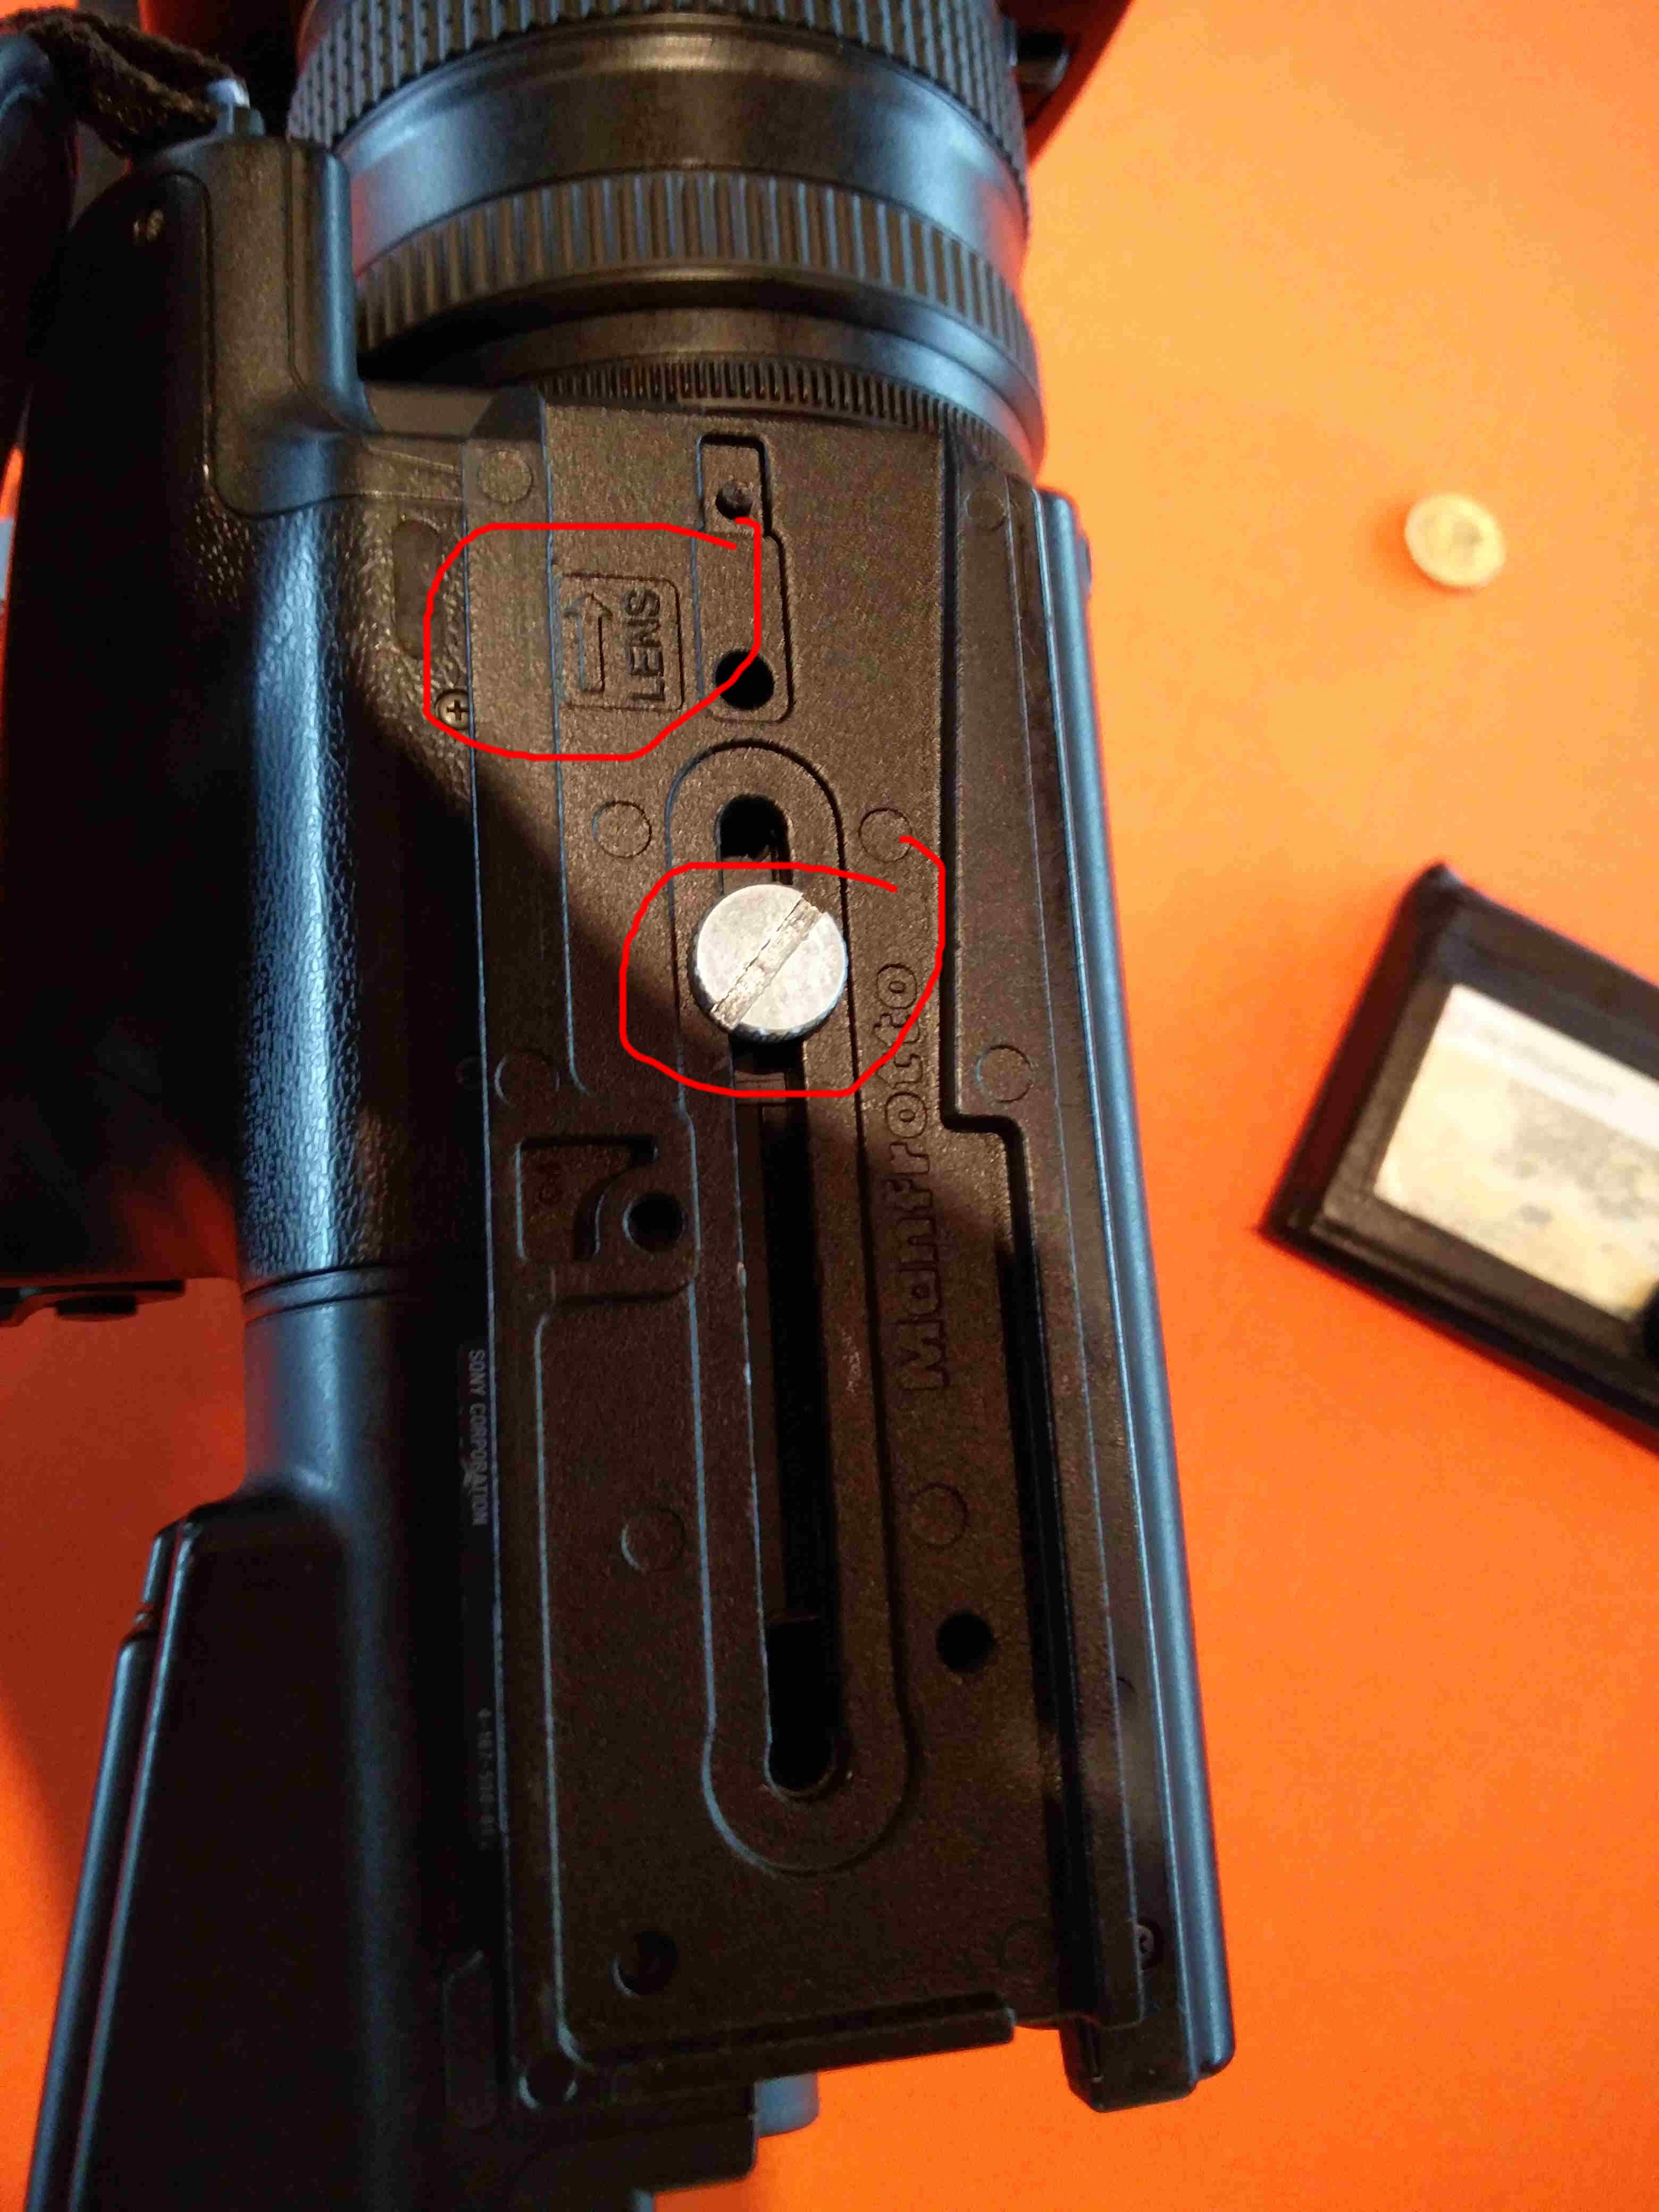
\includegraphics[width = 80mm]{Cam00.jpg}

\subsubsection{Plugging in power/HDMI}
First plug in the battery at the back, then plug in both the HDMI and the power cable. The entrance for both cables is next to each other right of the battery entrance. Look at the picture if you're unsure, make sure the FOSDEM video box has the other side of the HDMI cable.

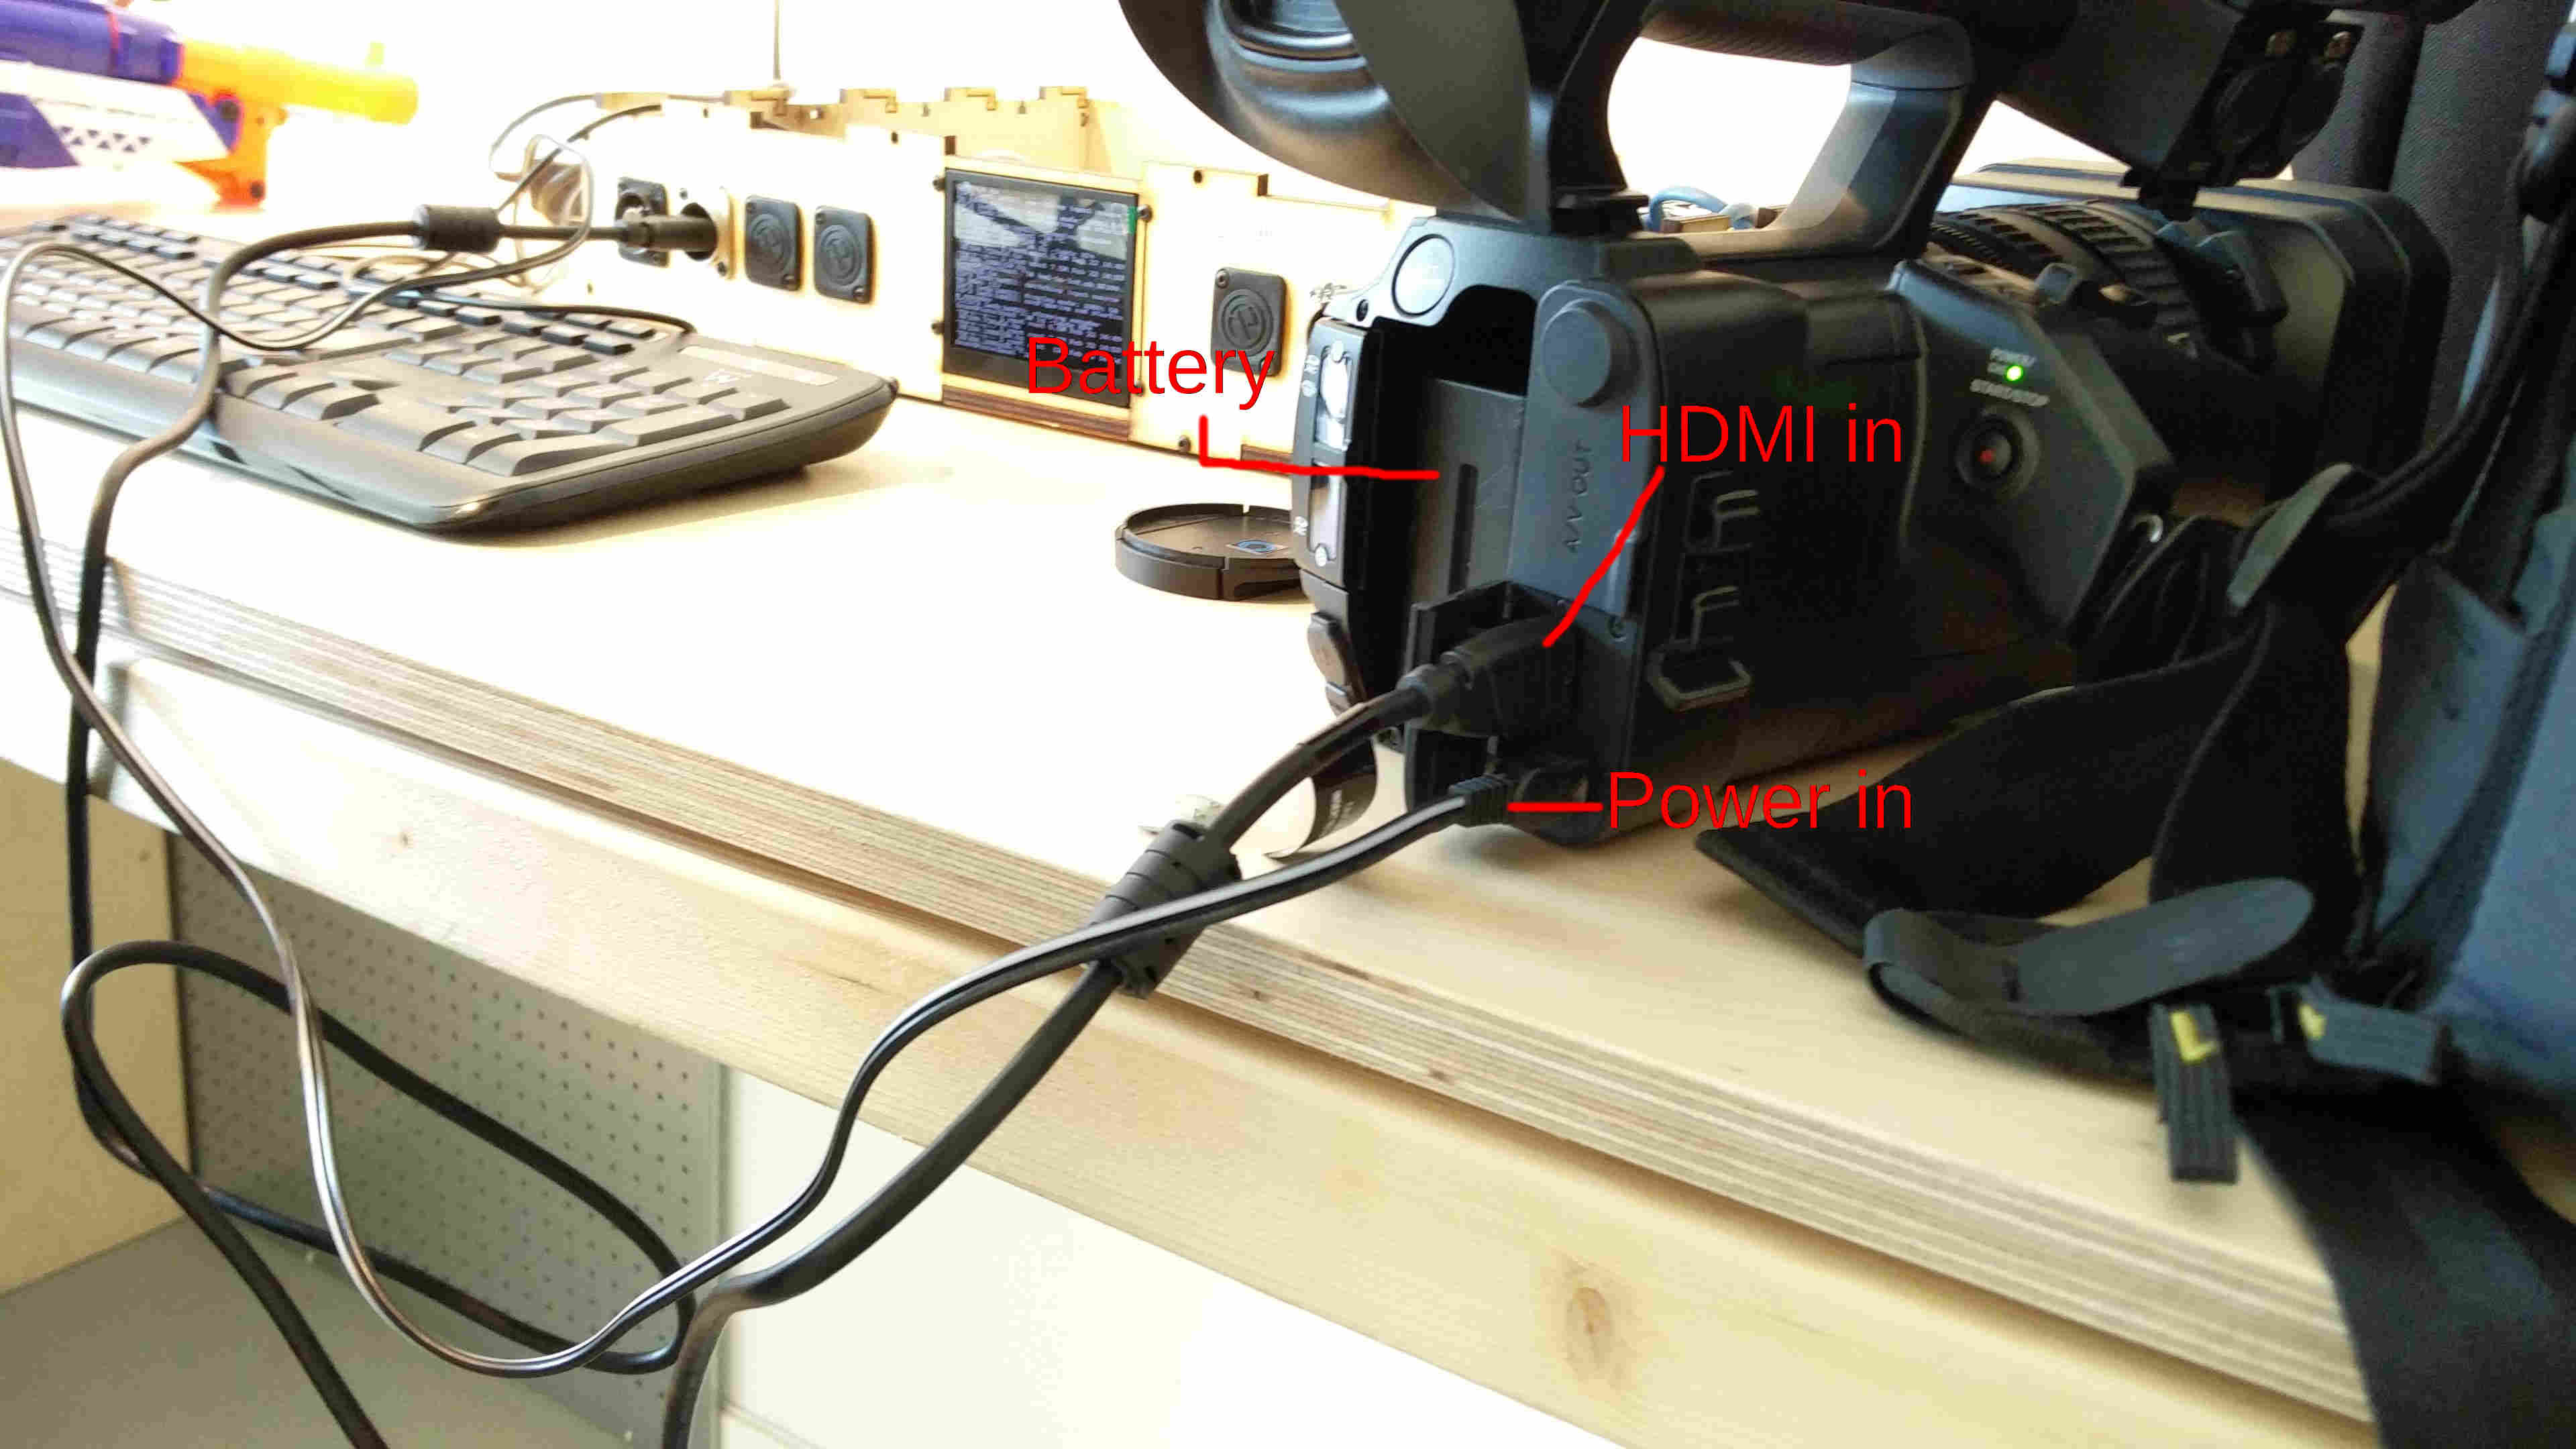
\includegraphics[width = 80mm]{Sony01.jpg}

\subsubsection{Pluggin in the Microphone}
Now plug in the XLR cable of the audio system in Input2.

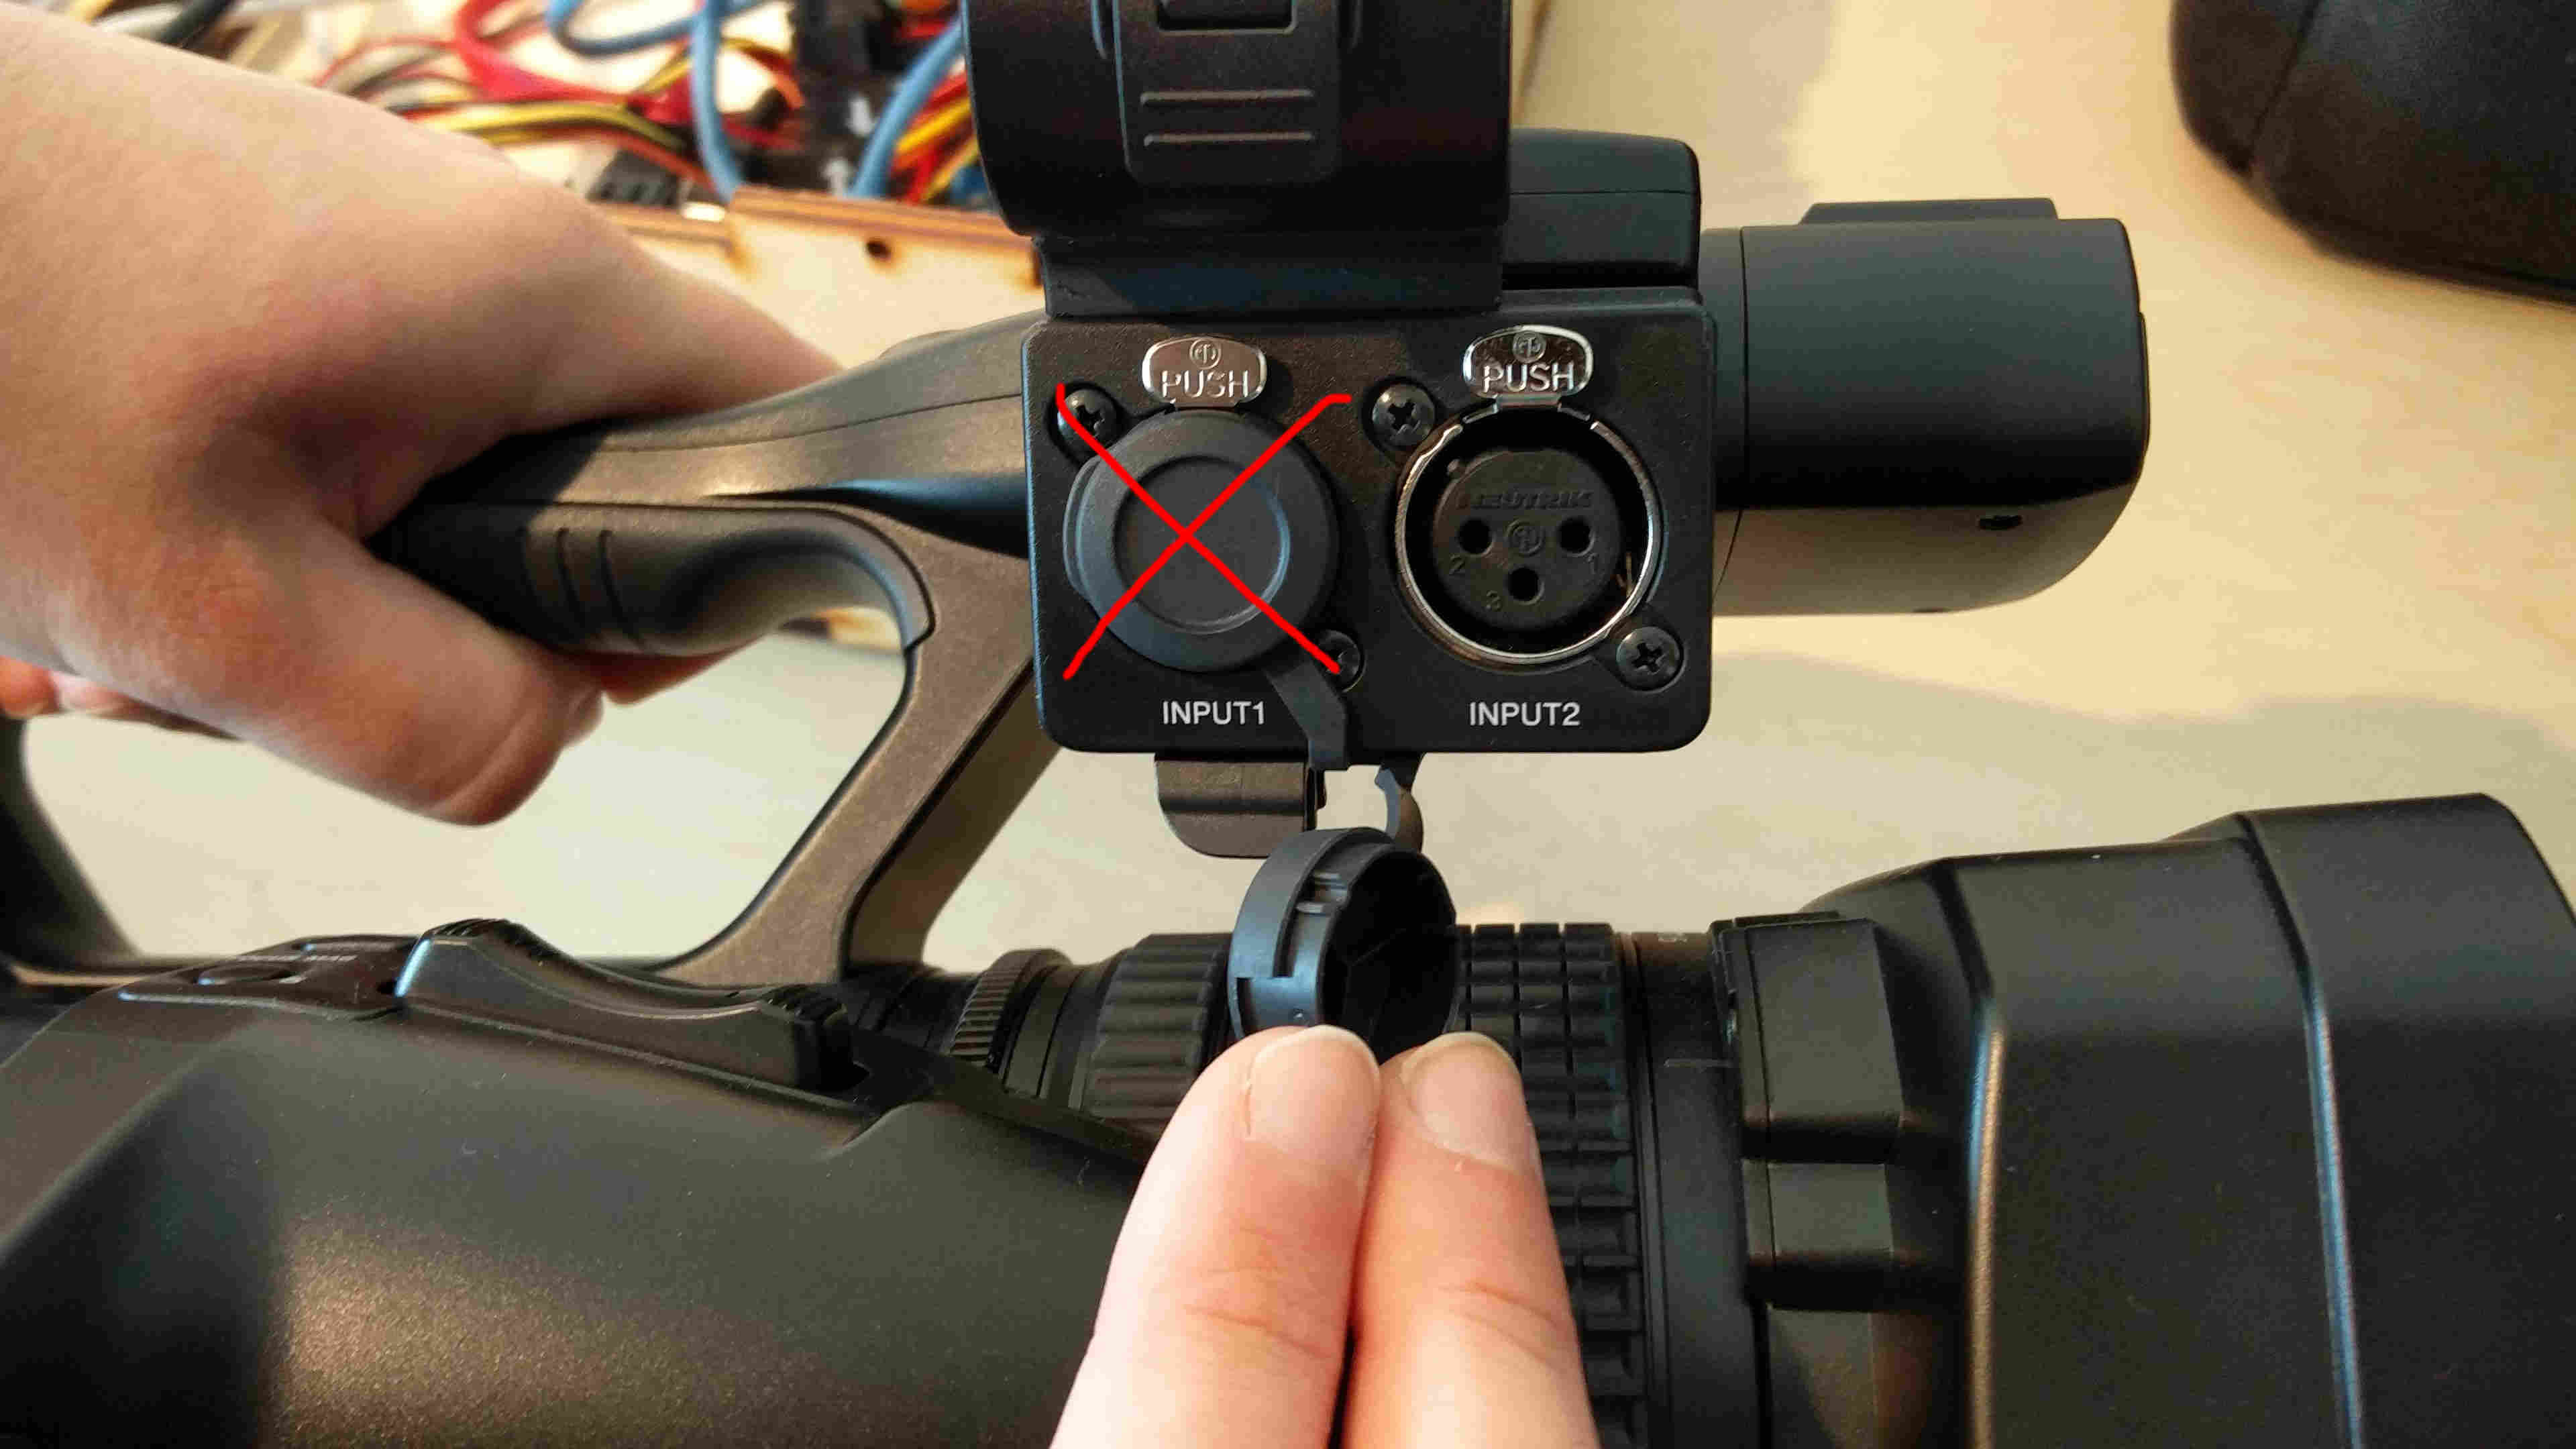
\includegraphics[width = 80mm]{Sony02.jpg}

\subsubsection{Turn on the camera}
You can find the power button at the left side of the camera (looking from behind). The power button is at the bottom of the side.

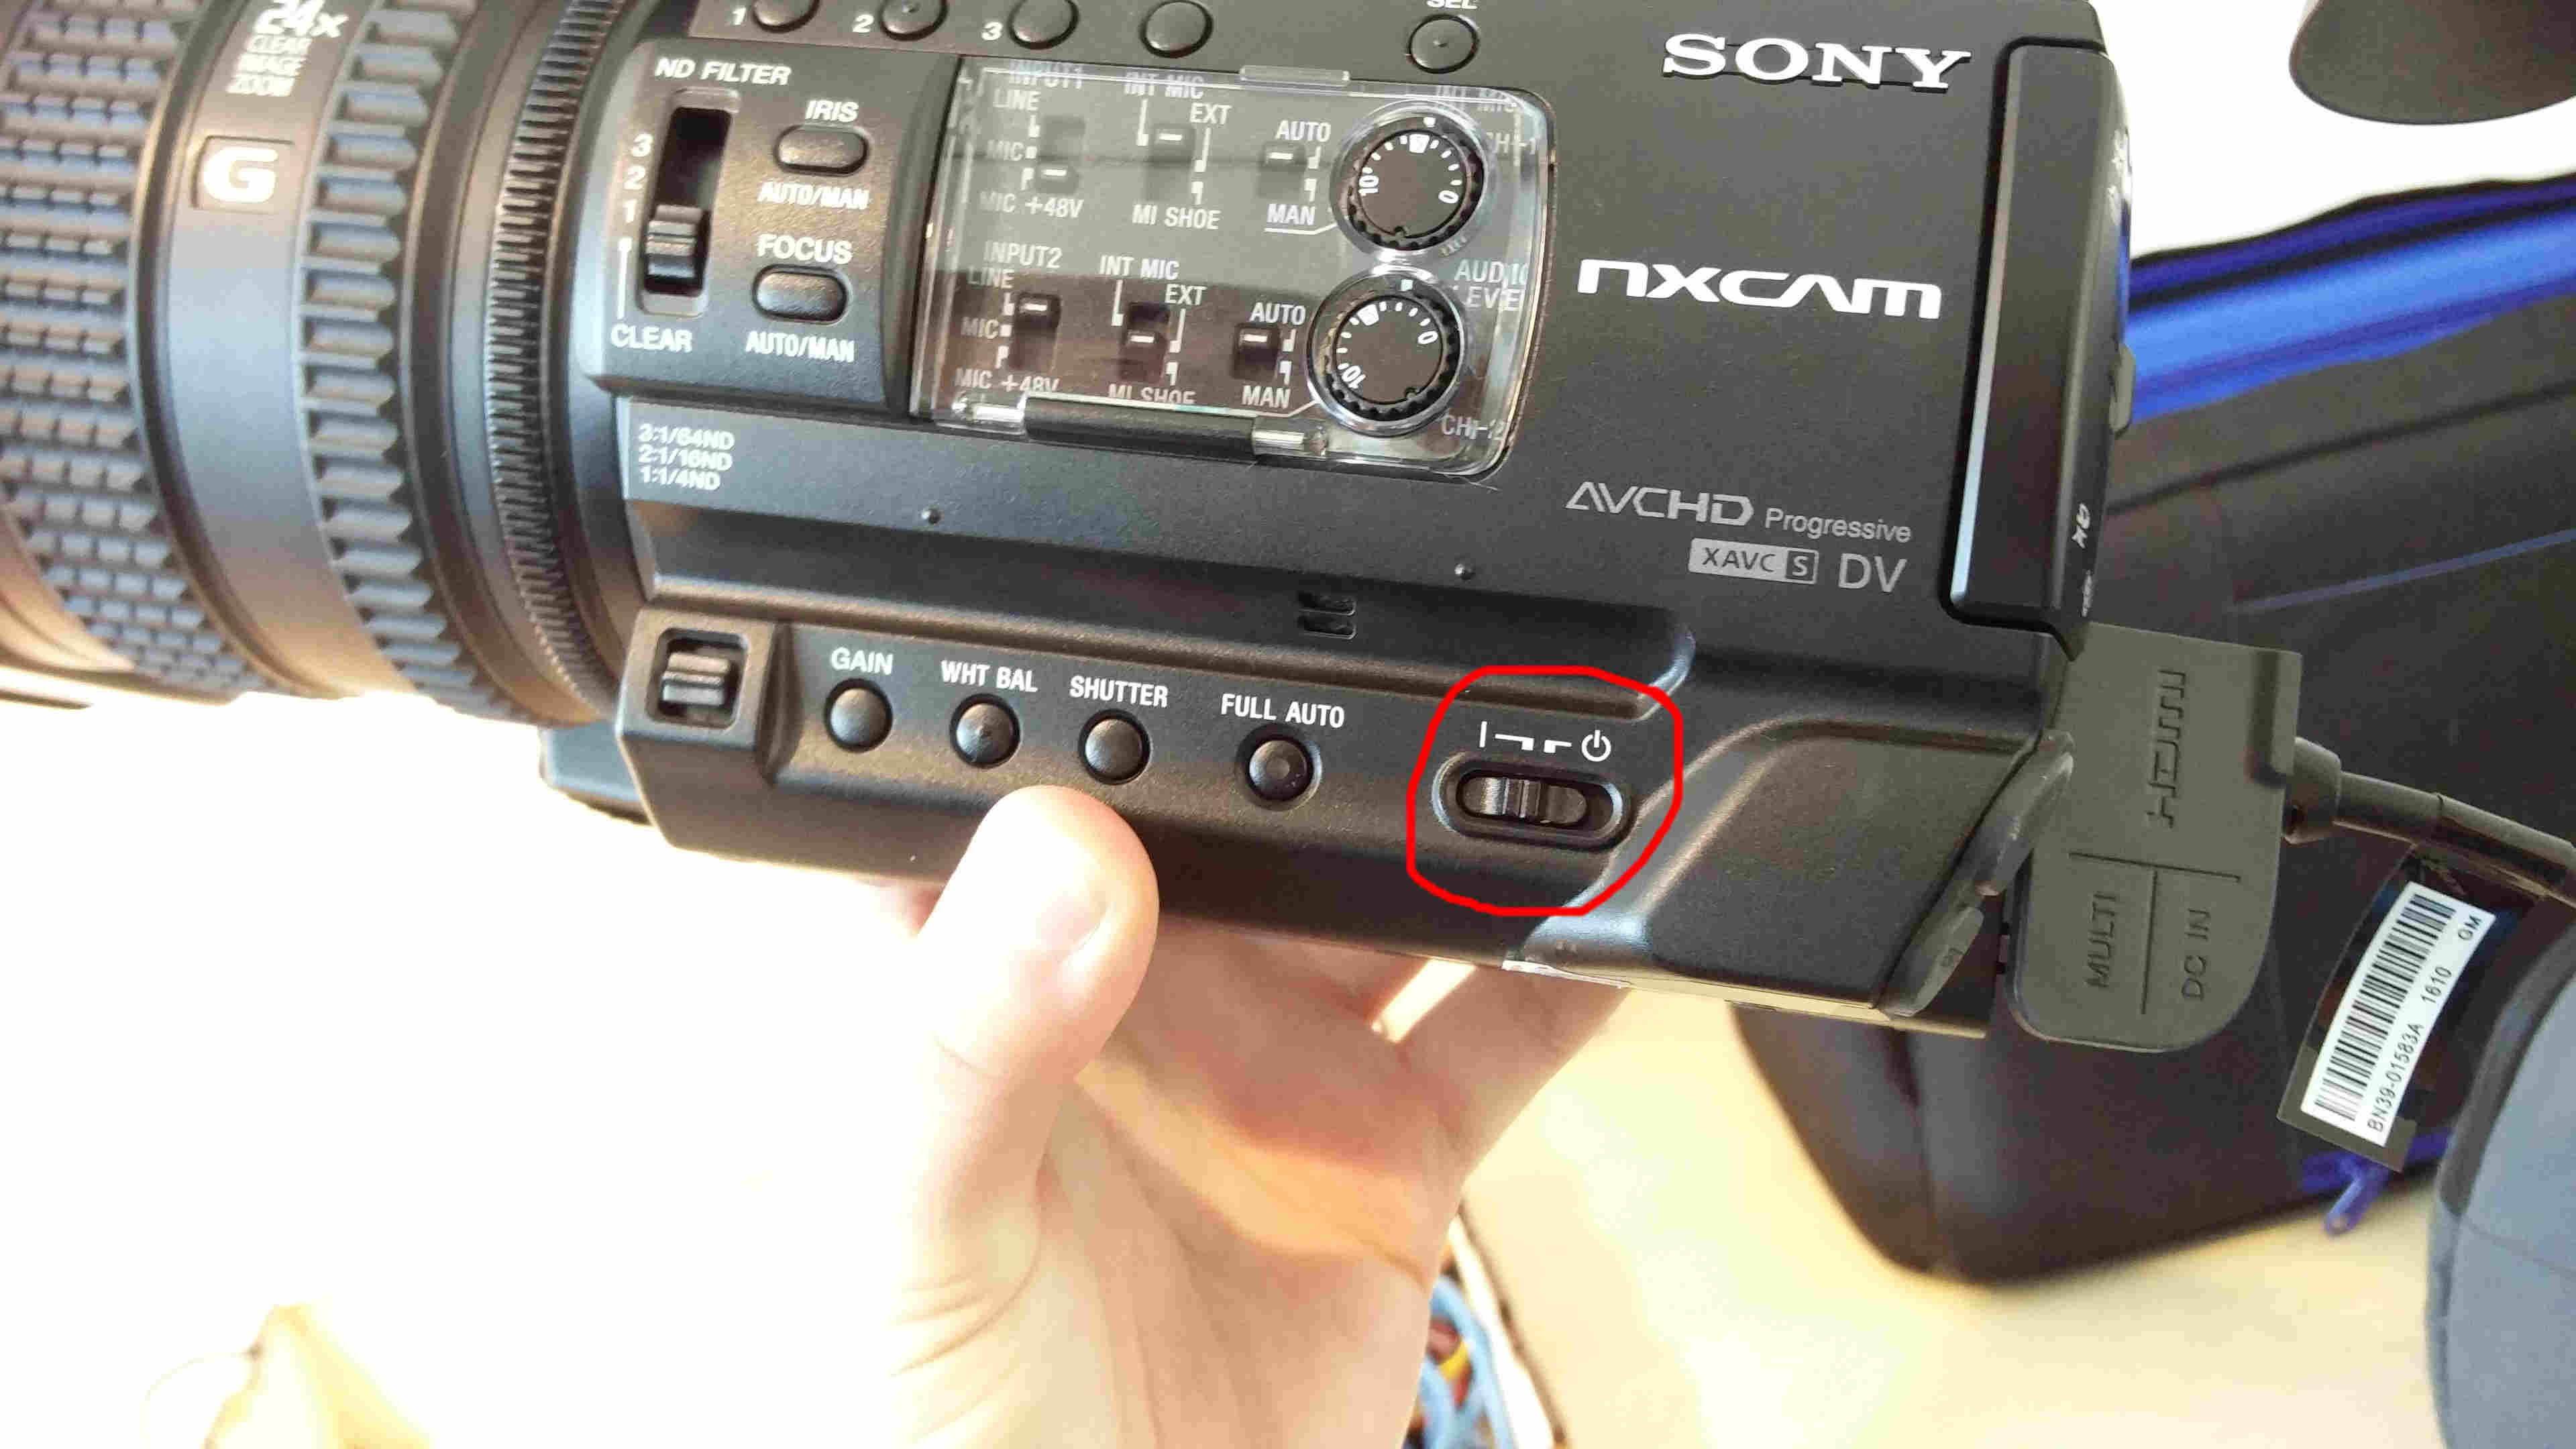
\includegraphics[width = 80mm]{Sony03.jpg}

\subsubsection{Audio settings}
The audio settings can only be done through the actual switches on the camera. Please verify if you've done them correctly with the image. The dial can be on any setting as the automatic setting of switch next to it overrides the dial.

\begin{tabular}{| l || l | l | l | l |}
Input & Left switch & Middle switch & Right switch & dial \\ \hline
Input1 & BOTTOM (Mic 48V) & TOP (INT MIC) & TOP (AUTO) & anything \\
Input2 & TOP (Line) & MIDDLE (EXT) & TOP (AUTO) & anything \\
\end{tabular}

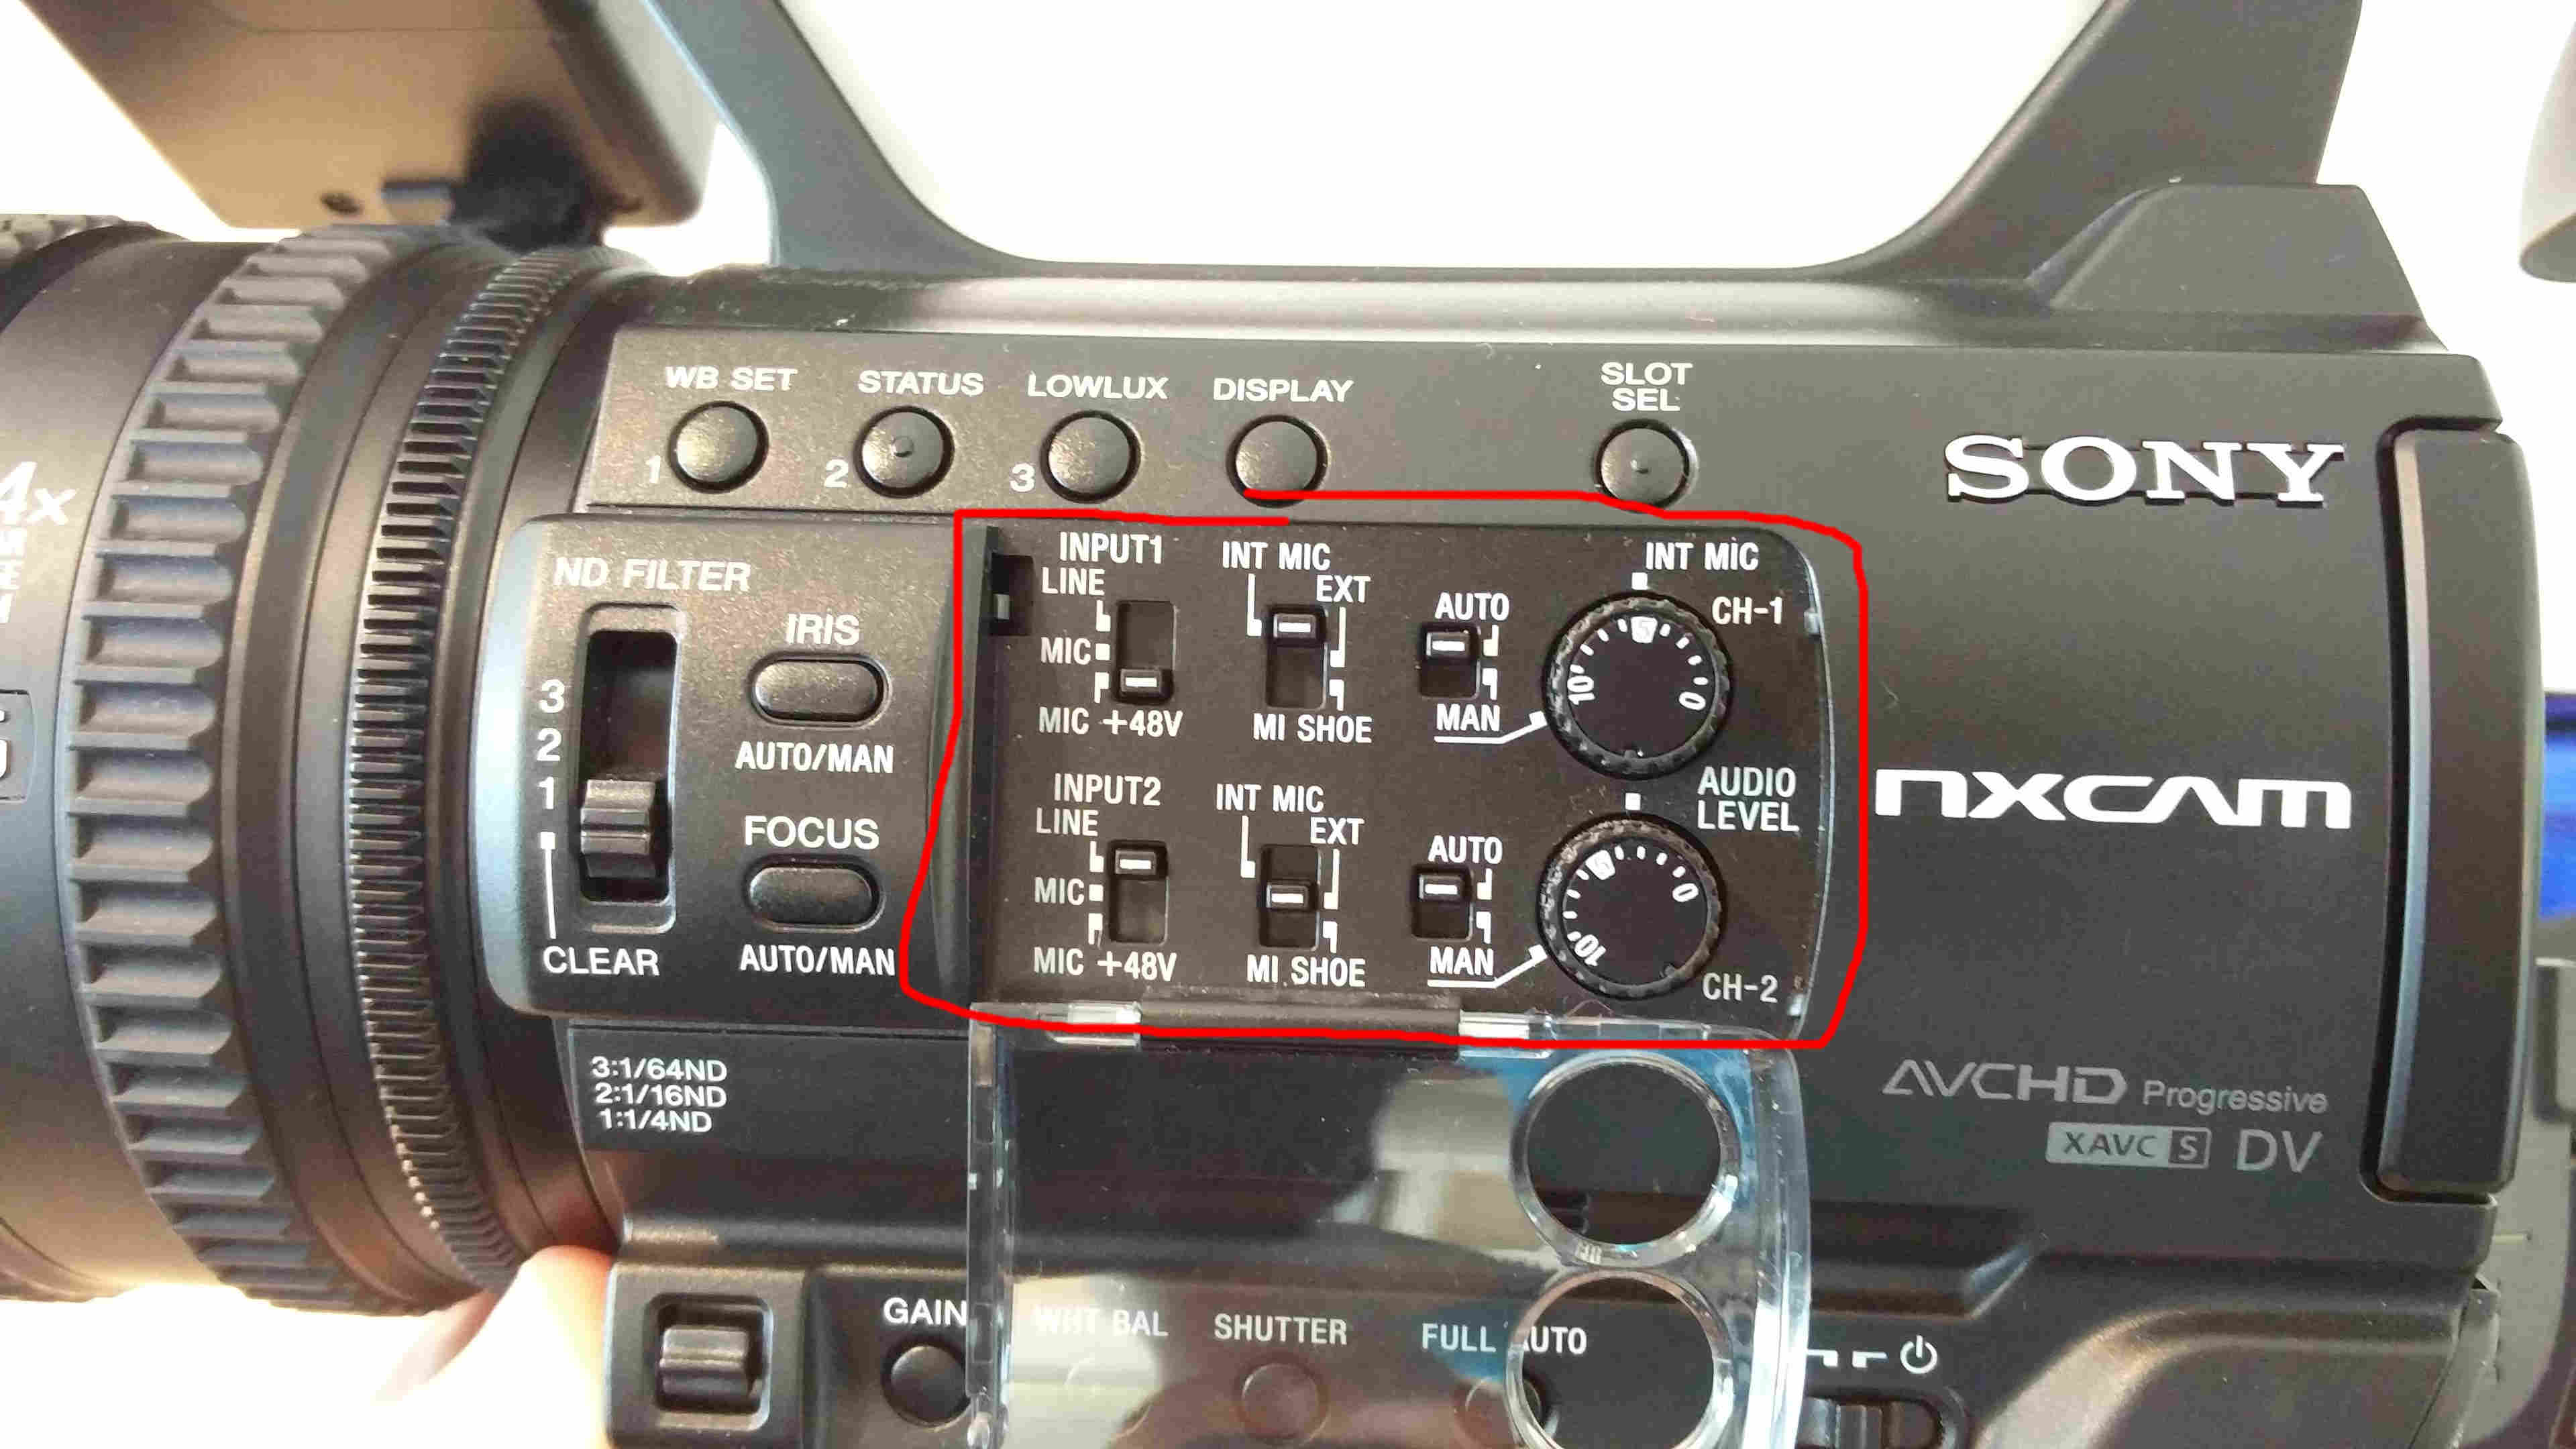
\includegraphics[width = 80mm]{Sony04.jpg}

\subsubsection{Video settings}
The video settings will be done through the onscreen display. The actually focussing and pointing the camera is not your task, it's fine to point it in the general direction afterwards.

You can set the video settings here:

Menu - 2nd Pictogram (2 arrows) - Video out - HDMI - Set to 720p.
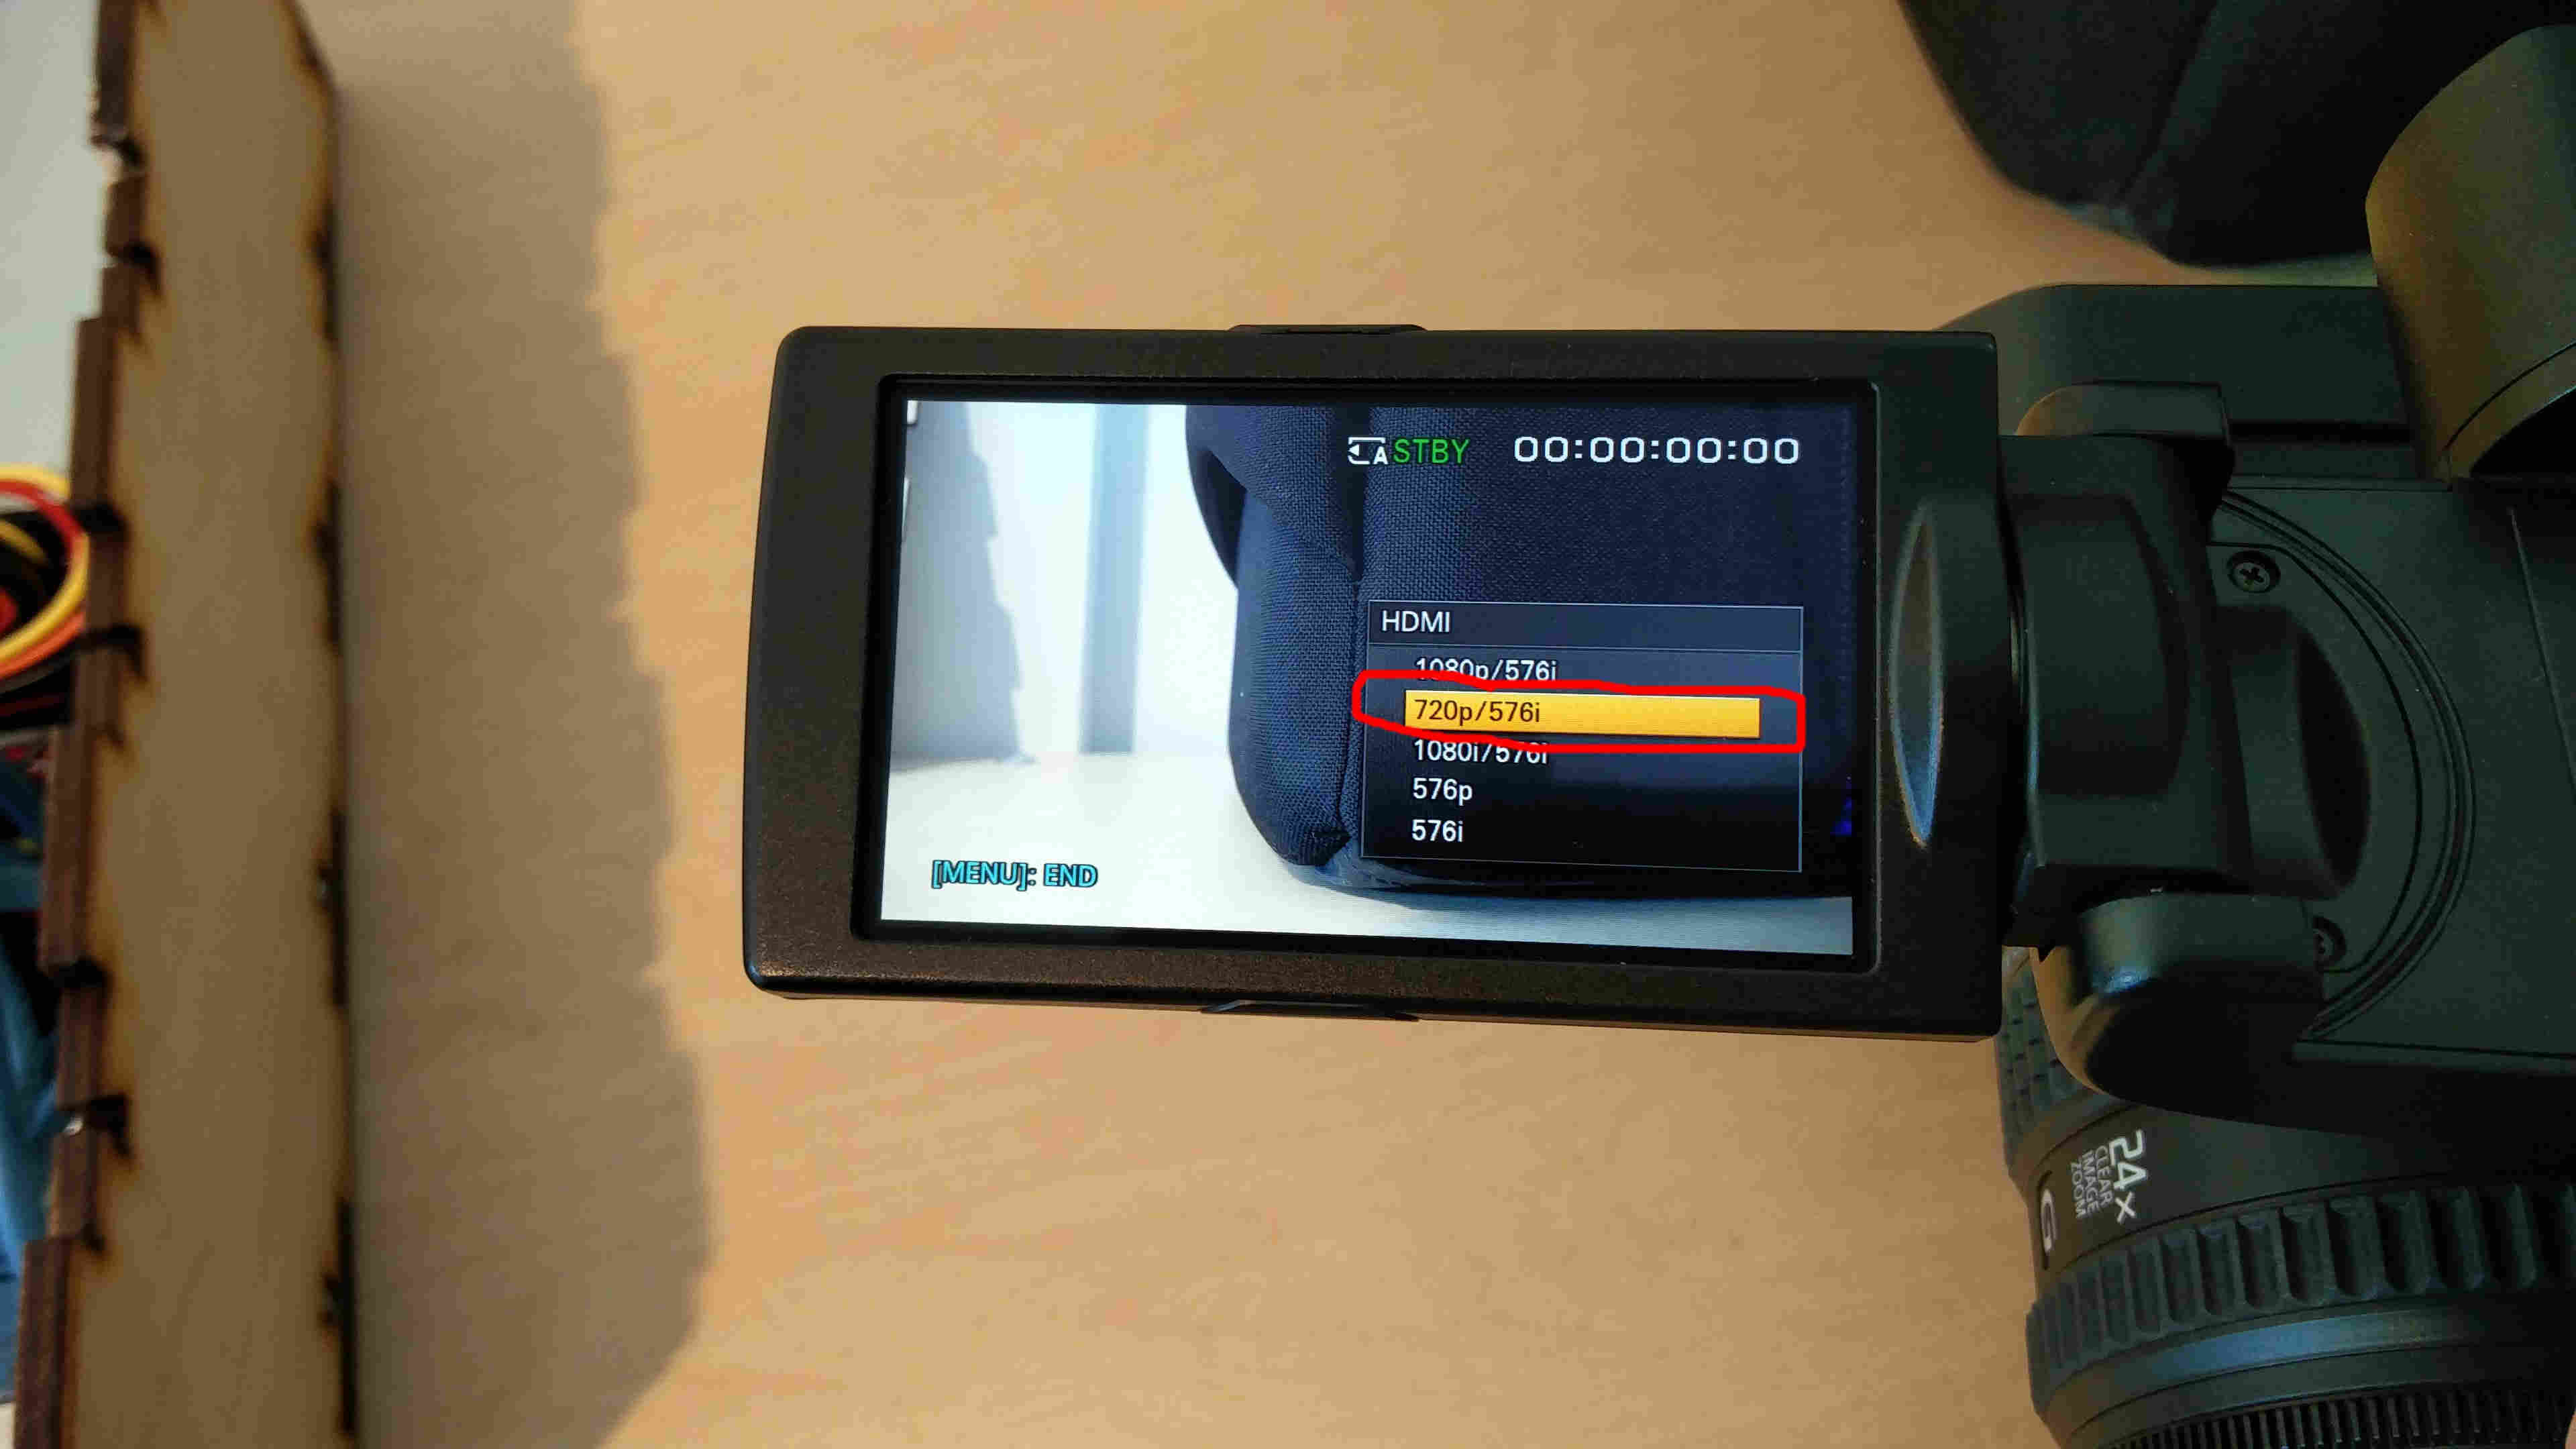
\includegraphics[width = 80mm]{Sony05.jpg}

Do note that the on screen display is for RECORDING, it doesn't show Video HDMI output except for when setting the option!
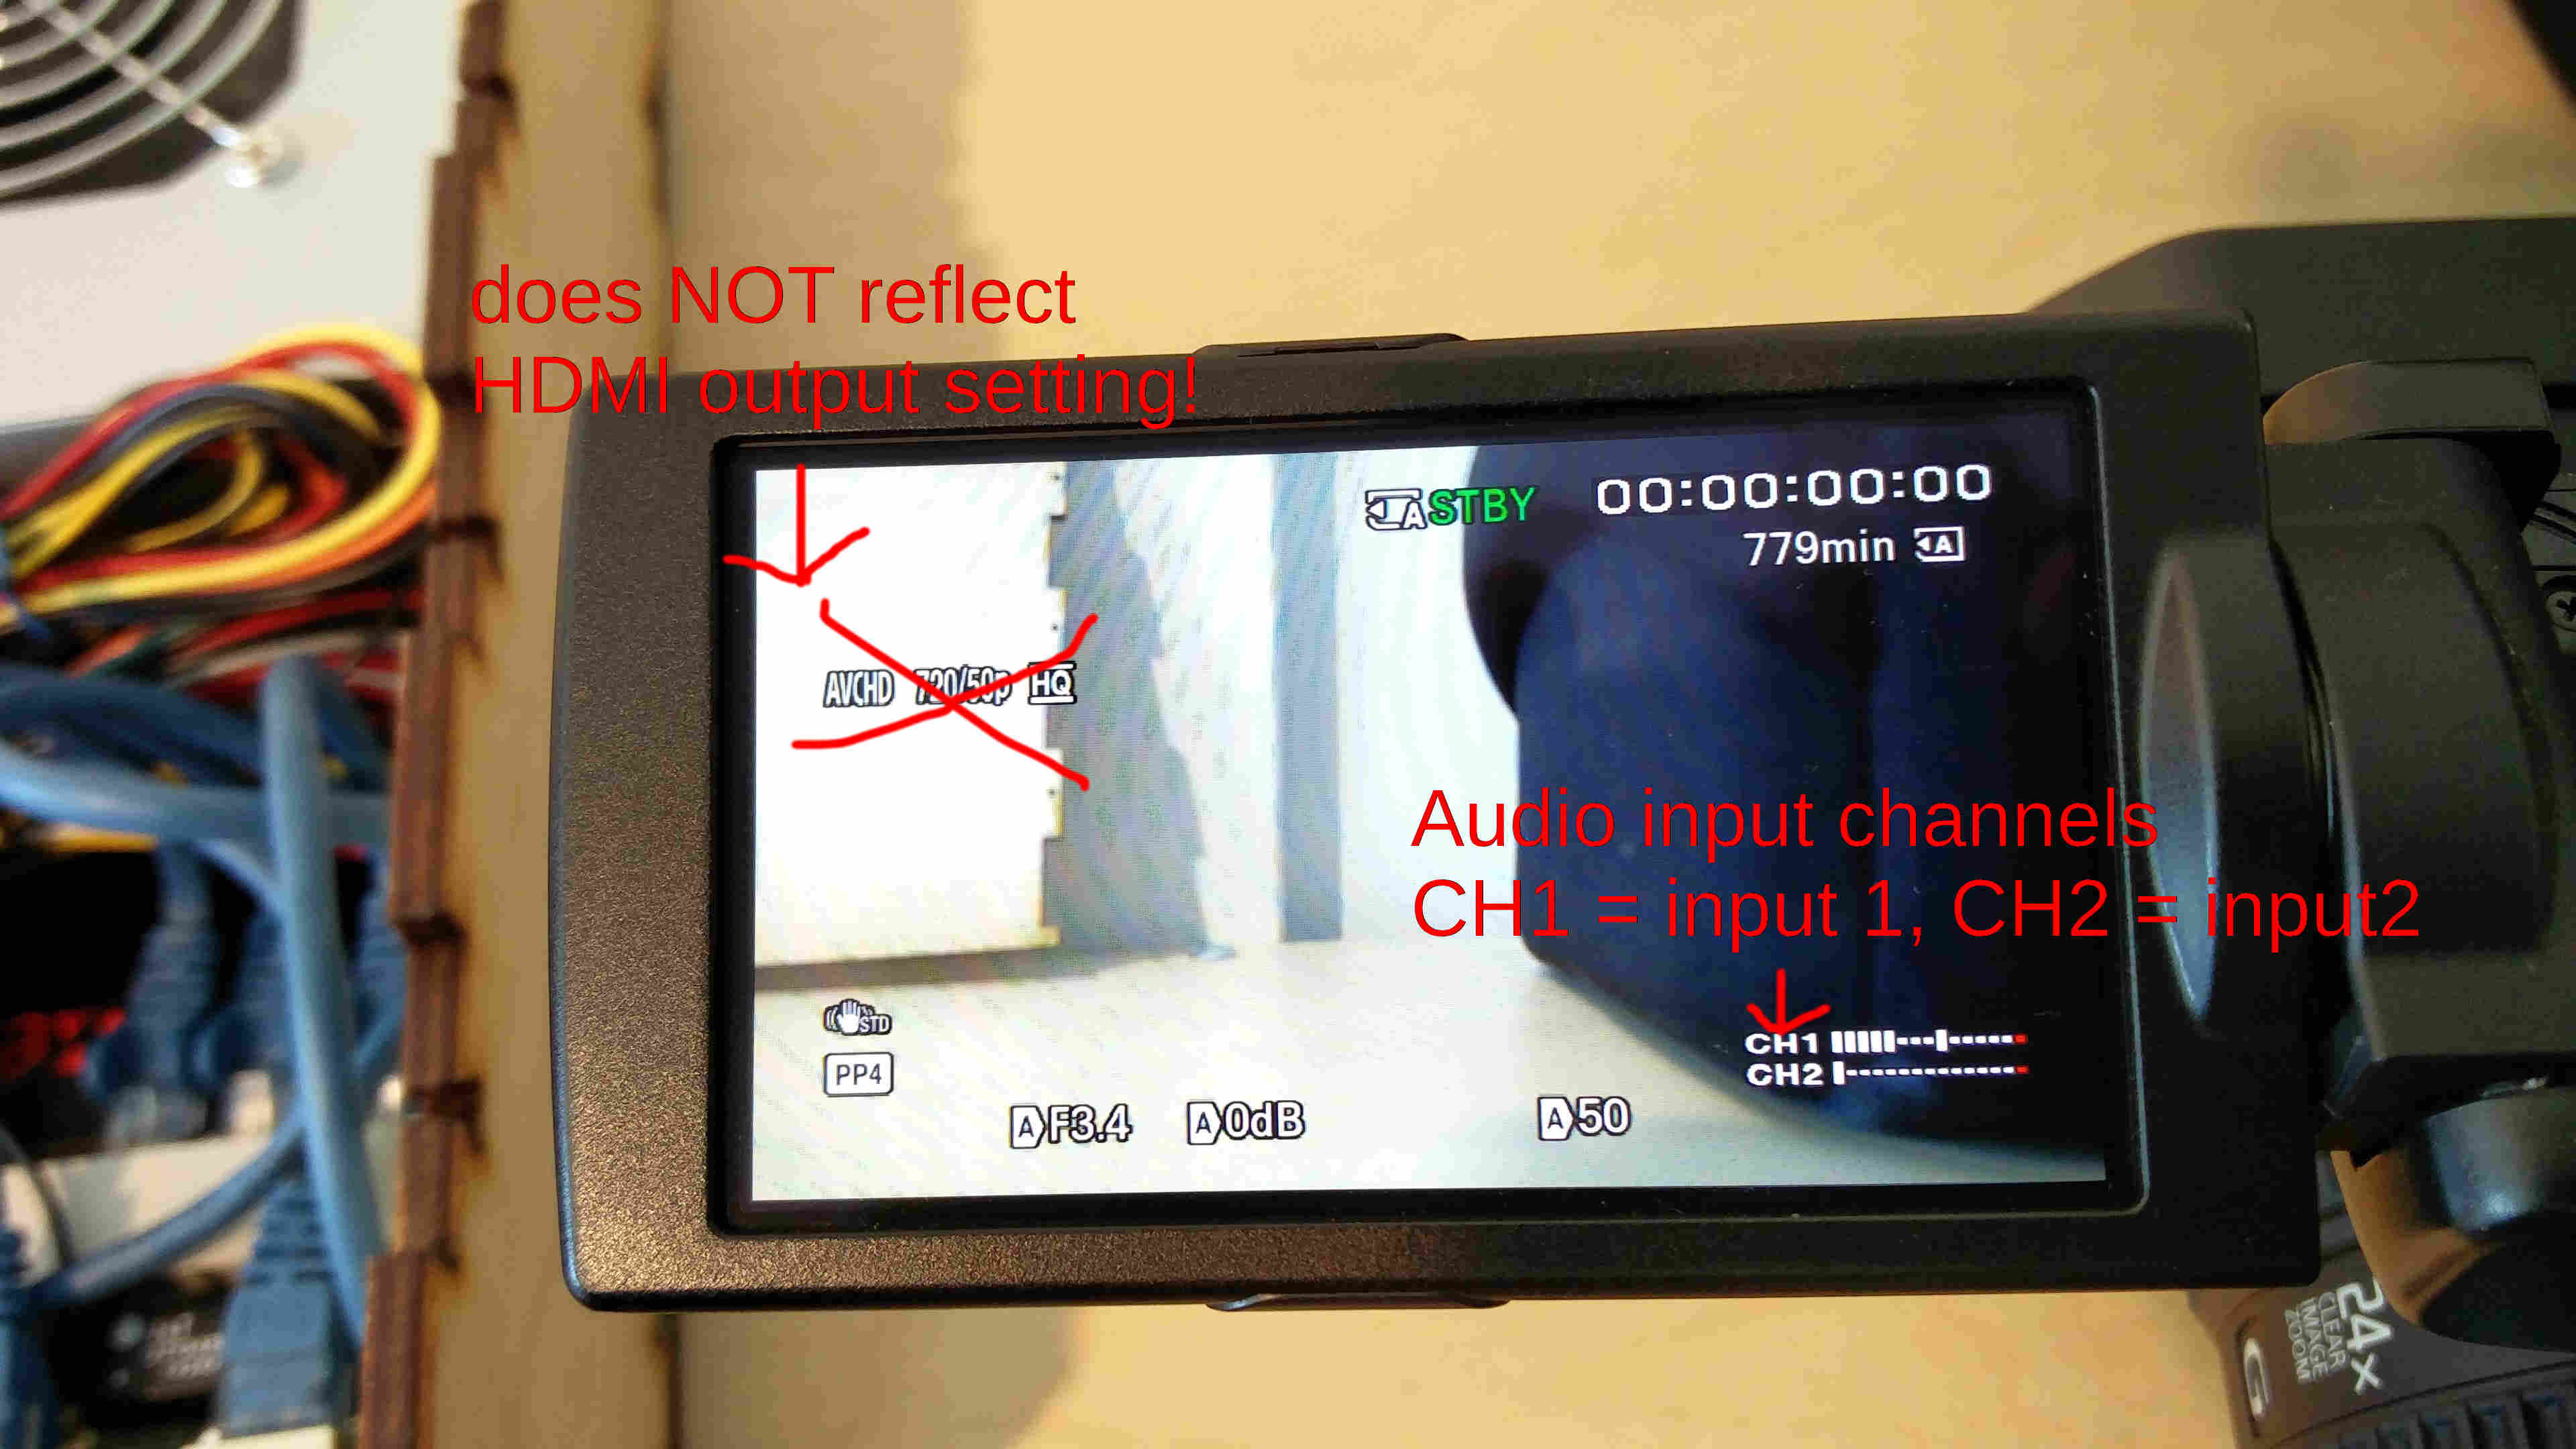
\includegraphics[width = 80mm]{Sony06.jpg}

\subsubsection{Remove the lens cover}
Remove the lens cover.

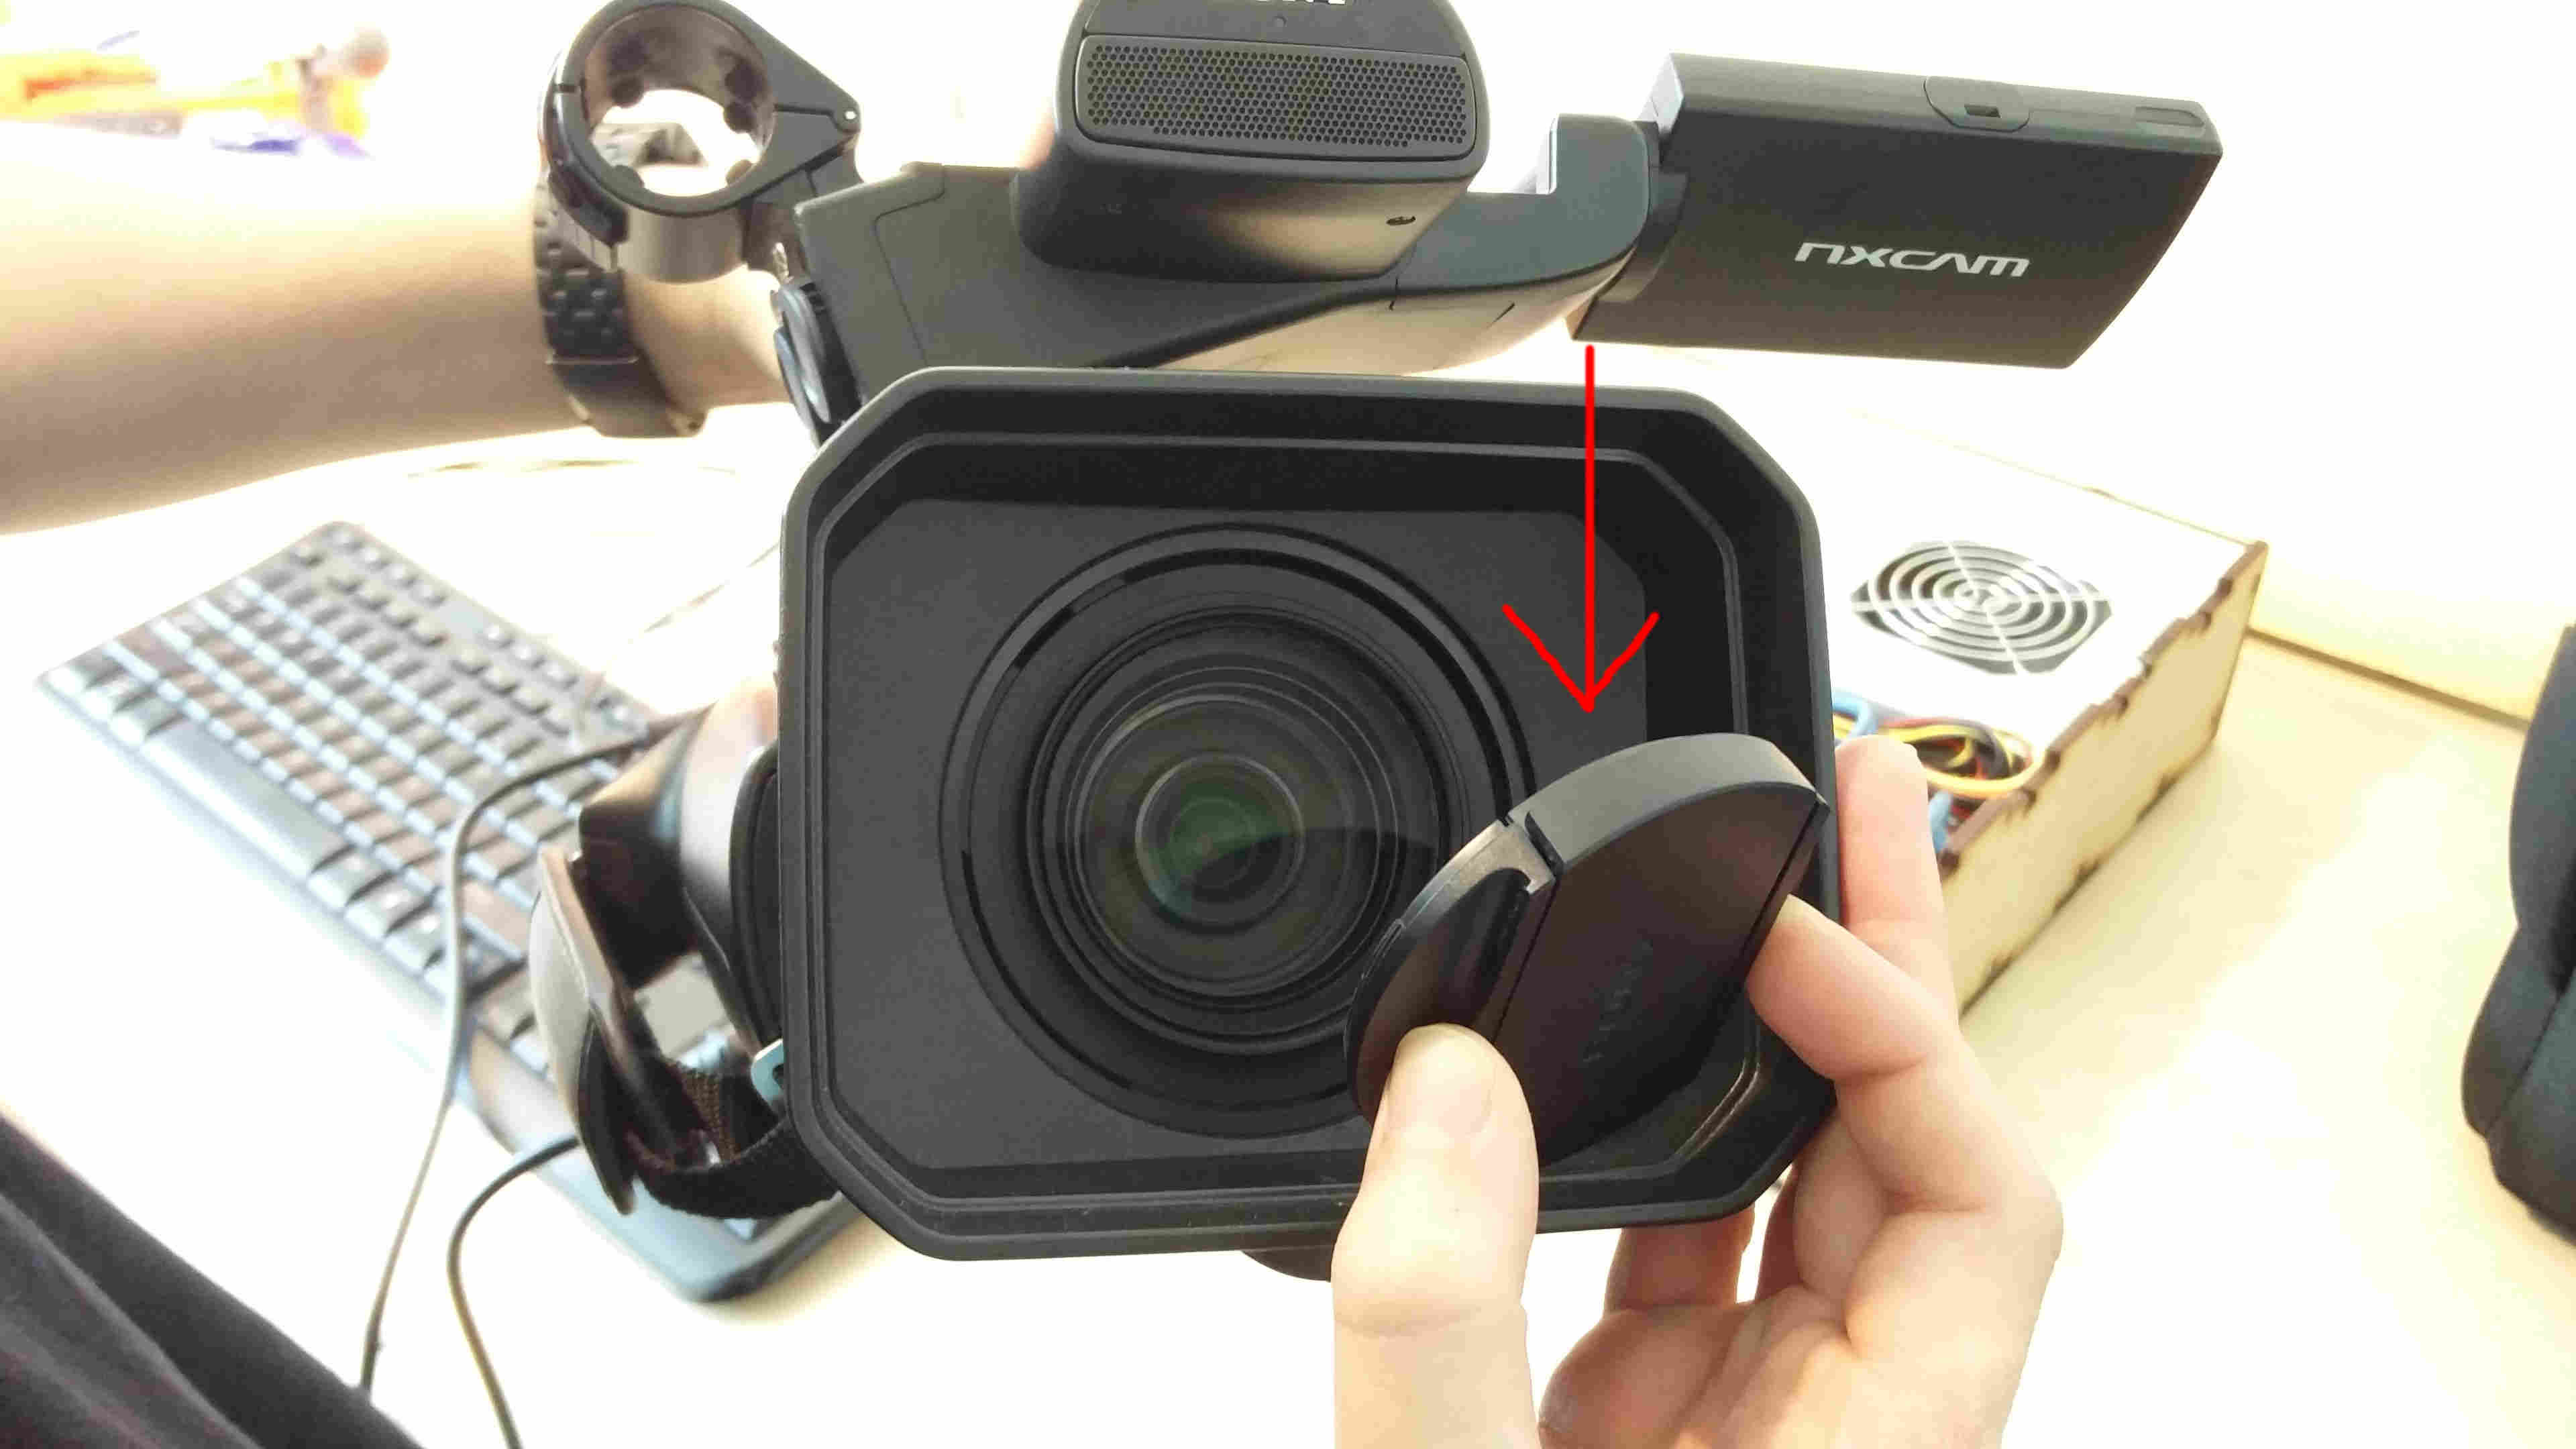
\includegraphics[width = 80mm]{Sony07.jpg}

\subsubsection{Double check}
Please check if the settings have been implemented correctly. 

For audio: you'll see CH1 spike when tapping the camera and CH2 when tapping the speaker microphone, do note that the speaker microphone will have to be turned on for this to work. Alternatively you can grab a headset and CH1 should come out of the left ear and CH2 should come out of the right ear.

For video: You'll have to reopen the settings and see if they're still at the correct settings: 1280x720 
with 50p refreshrate.

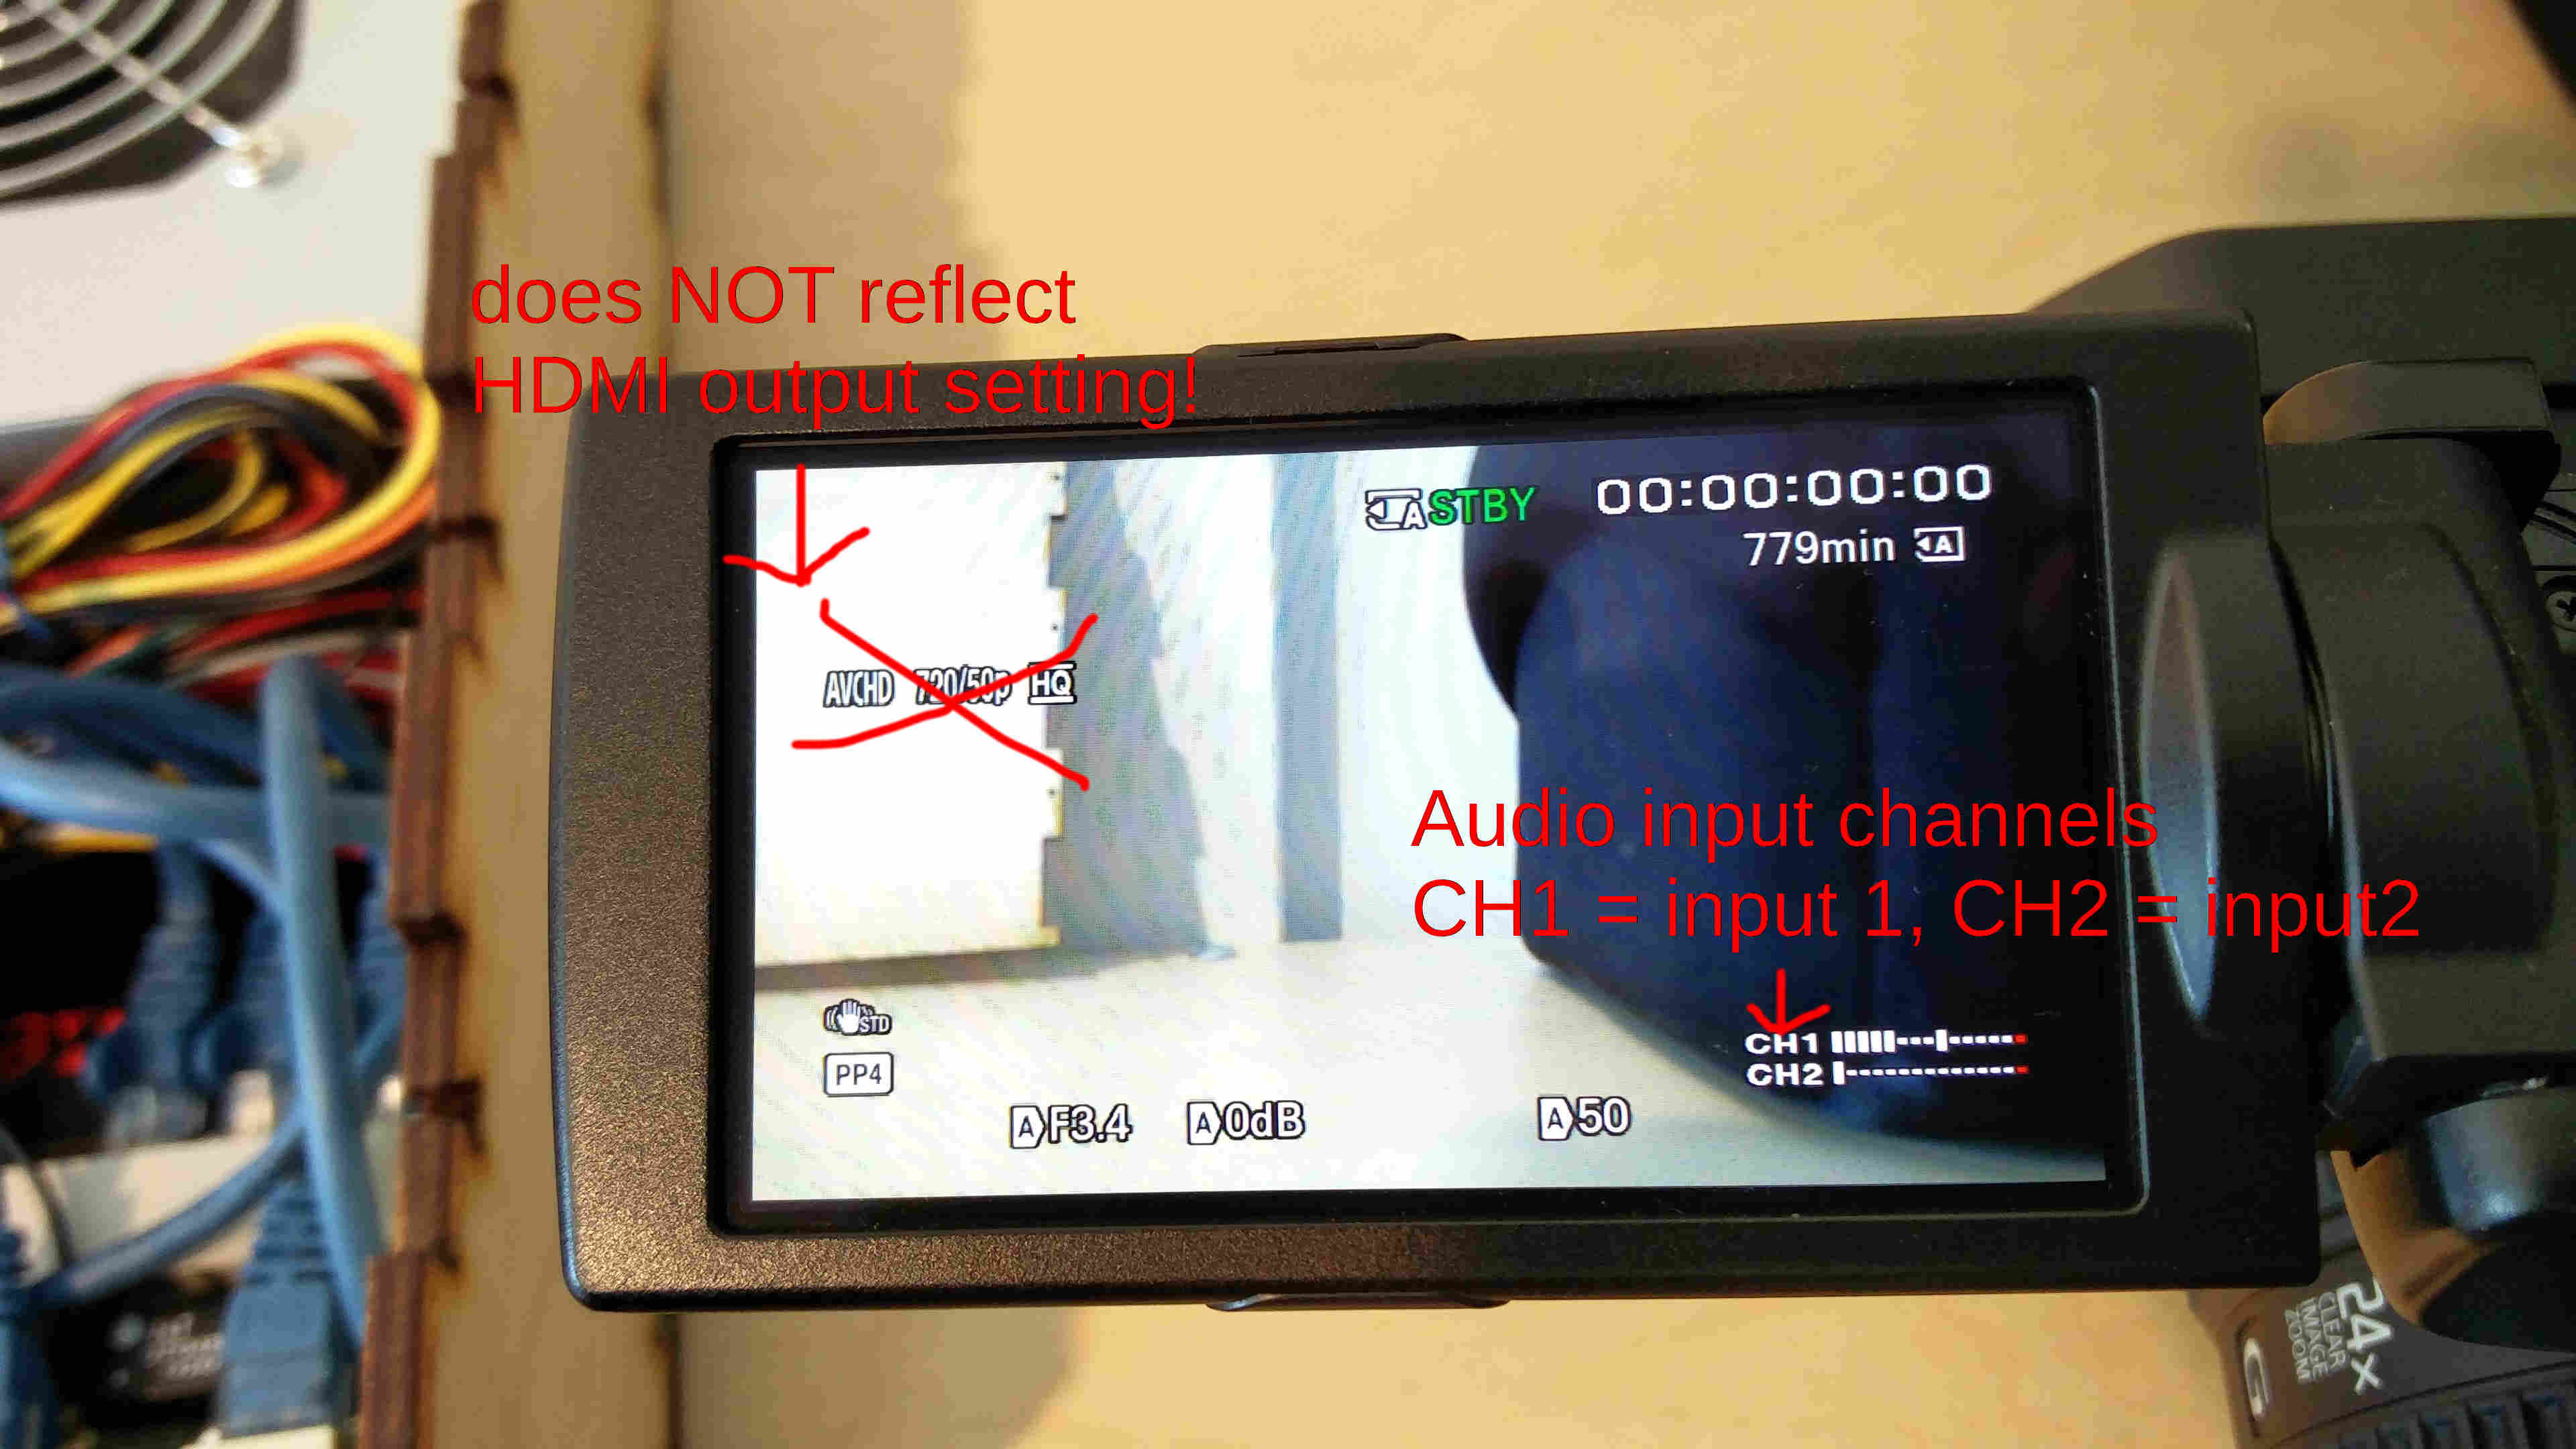
\includegraphics[width = 80mm]{Sony06.jpg}

\subsubsection{Contact control}
Please report that you've finished the room at the assigned control points. They will have the follow-up steps and know what still has to be done in the building.

\subsection{Correct camera set up Canon XF100E}

\subsubsection{Screw camera on mount}
Screw the camera on the tri-pod. Every camera has a screw hole at the bottom that can be used for this. The plate has a distinct point camera in this direction arrow, pay attention to it. The screw can be tightened by a coin or anything coinsized.

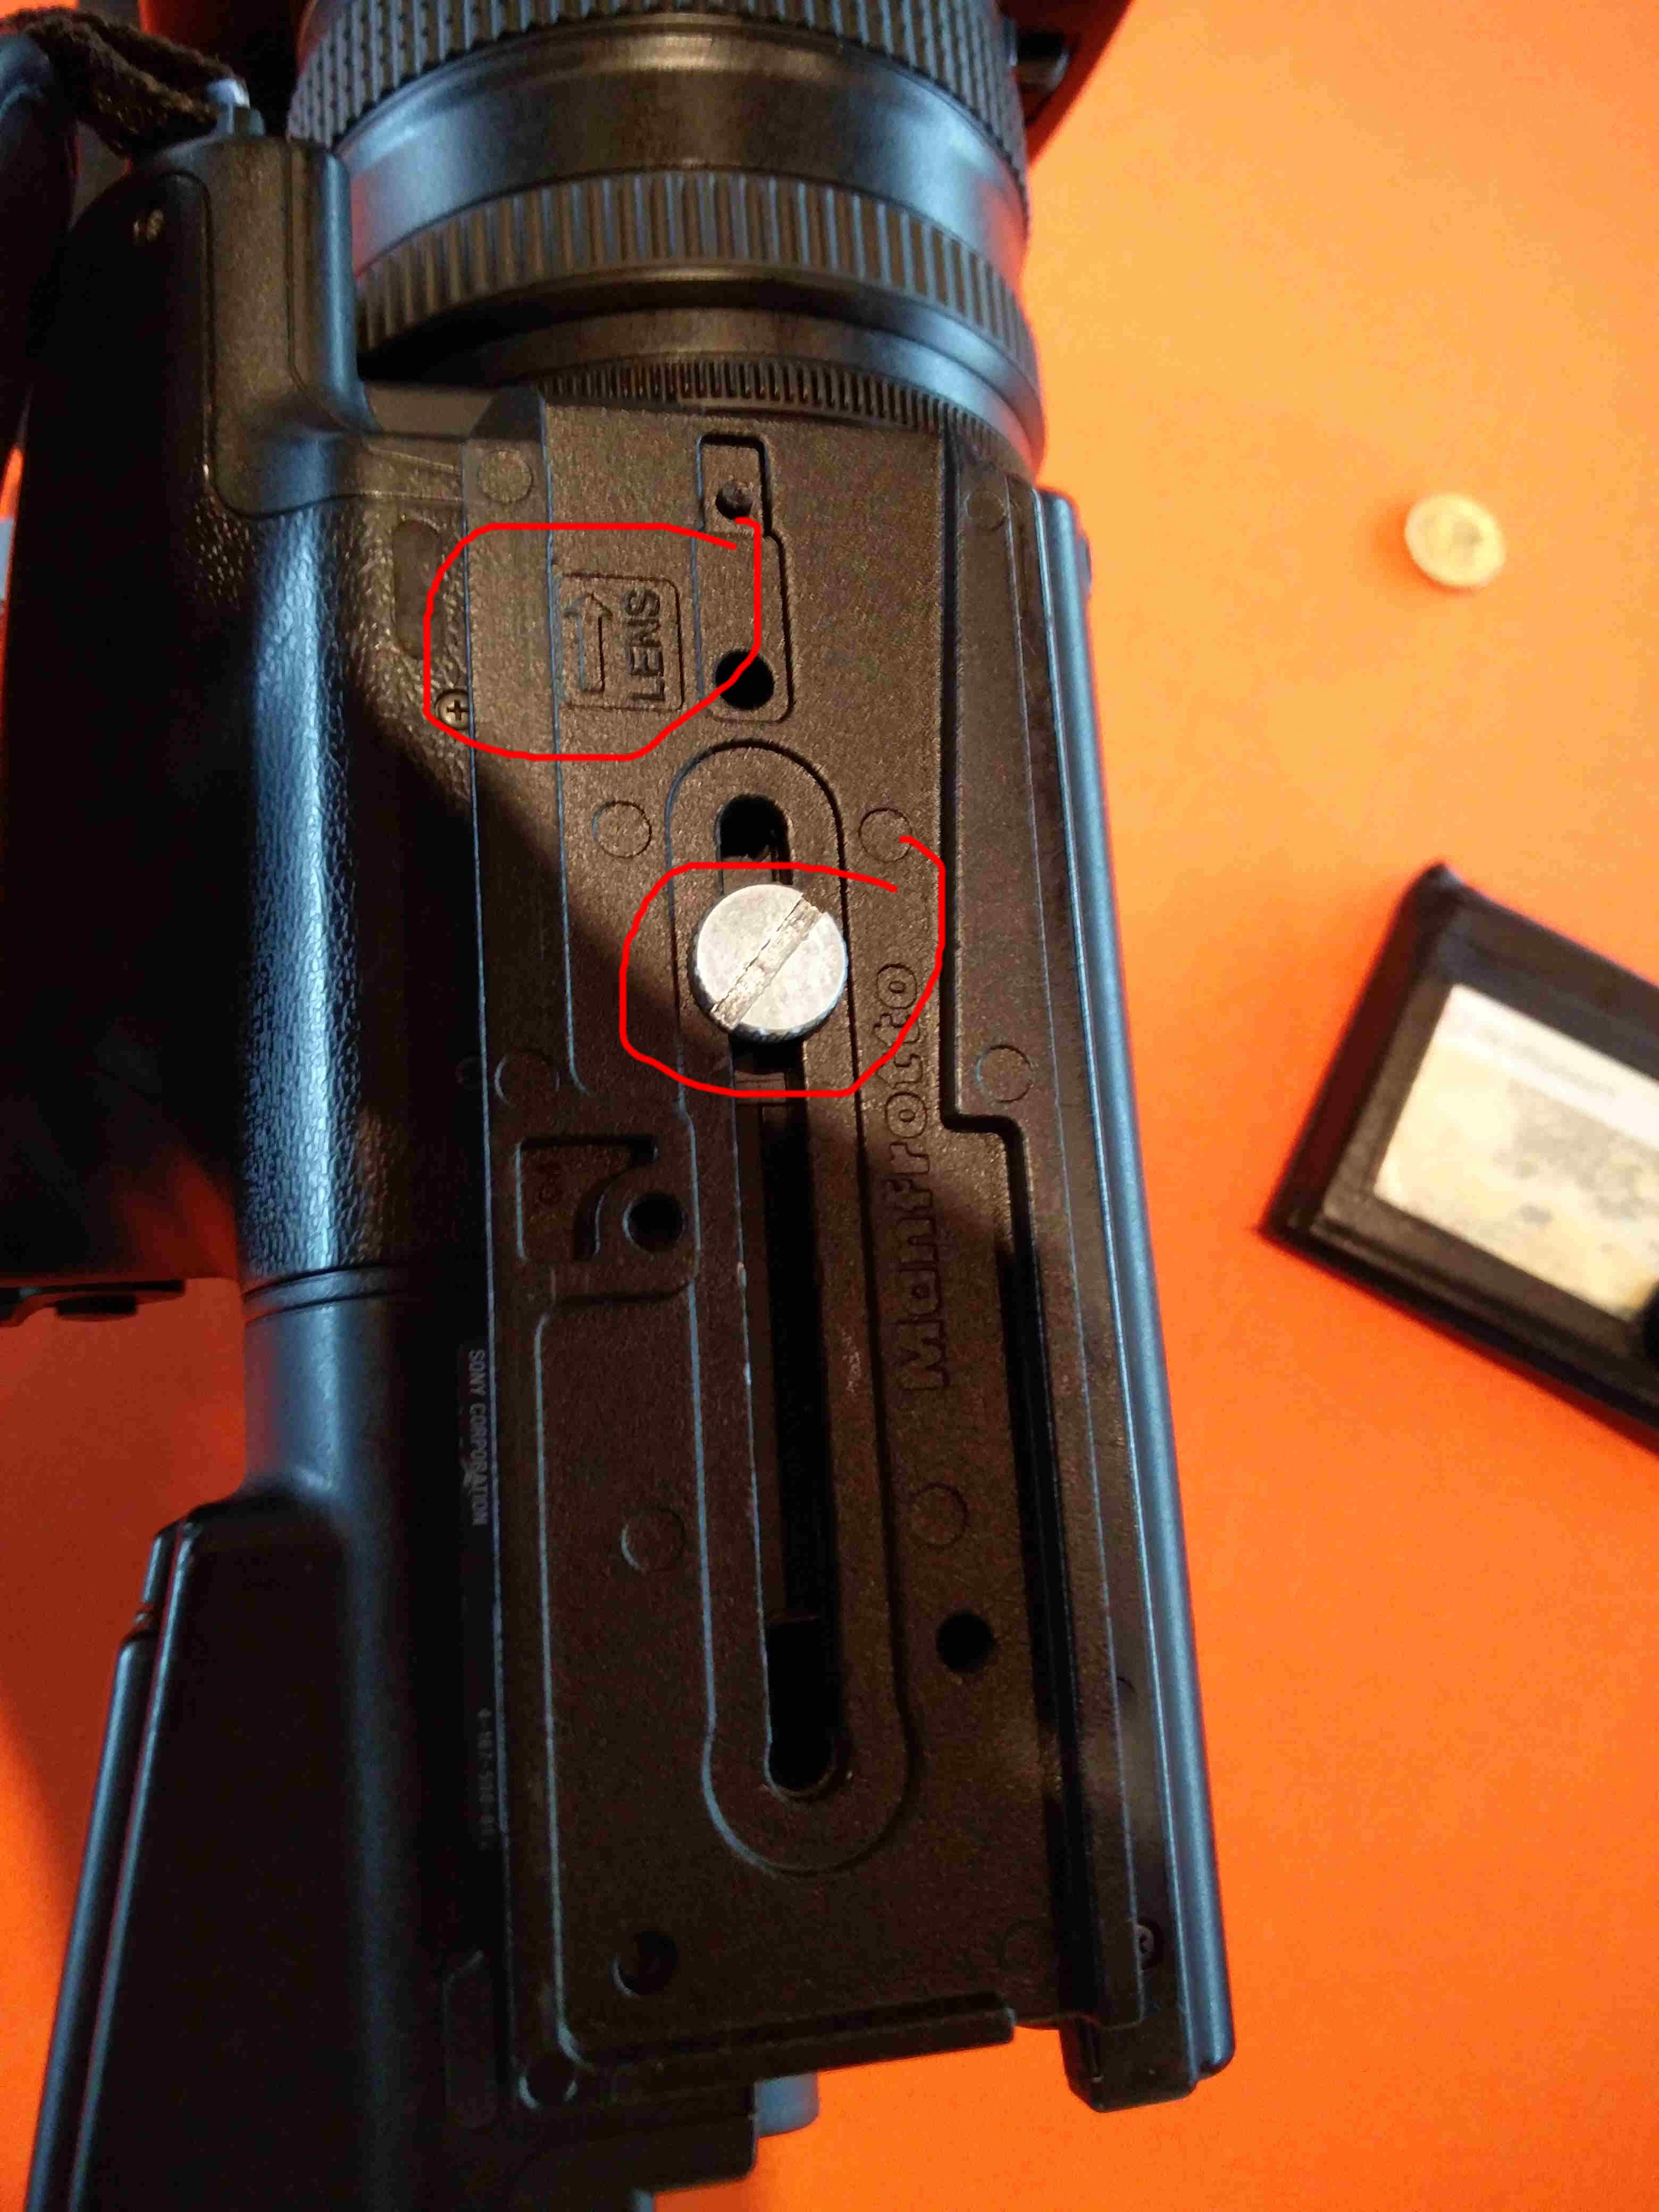
\includegraphics[width = 80mm]{Cam00.jpg}

\subsubsection{Plugging in power/HDMI}
First plug in the battery at the back, then plug in both the HDMI and the power cable. The HDMI is hidden at the side, the power is at the back, left of the battery labled Power Source. make sure the FOSDEM video box has the other side of the HDMI cable.

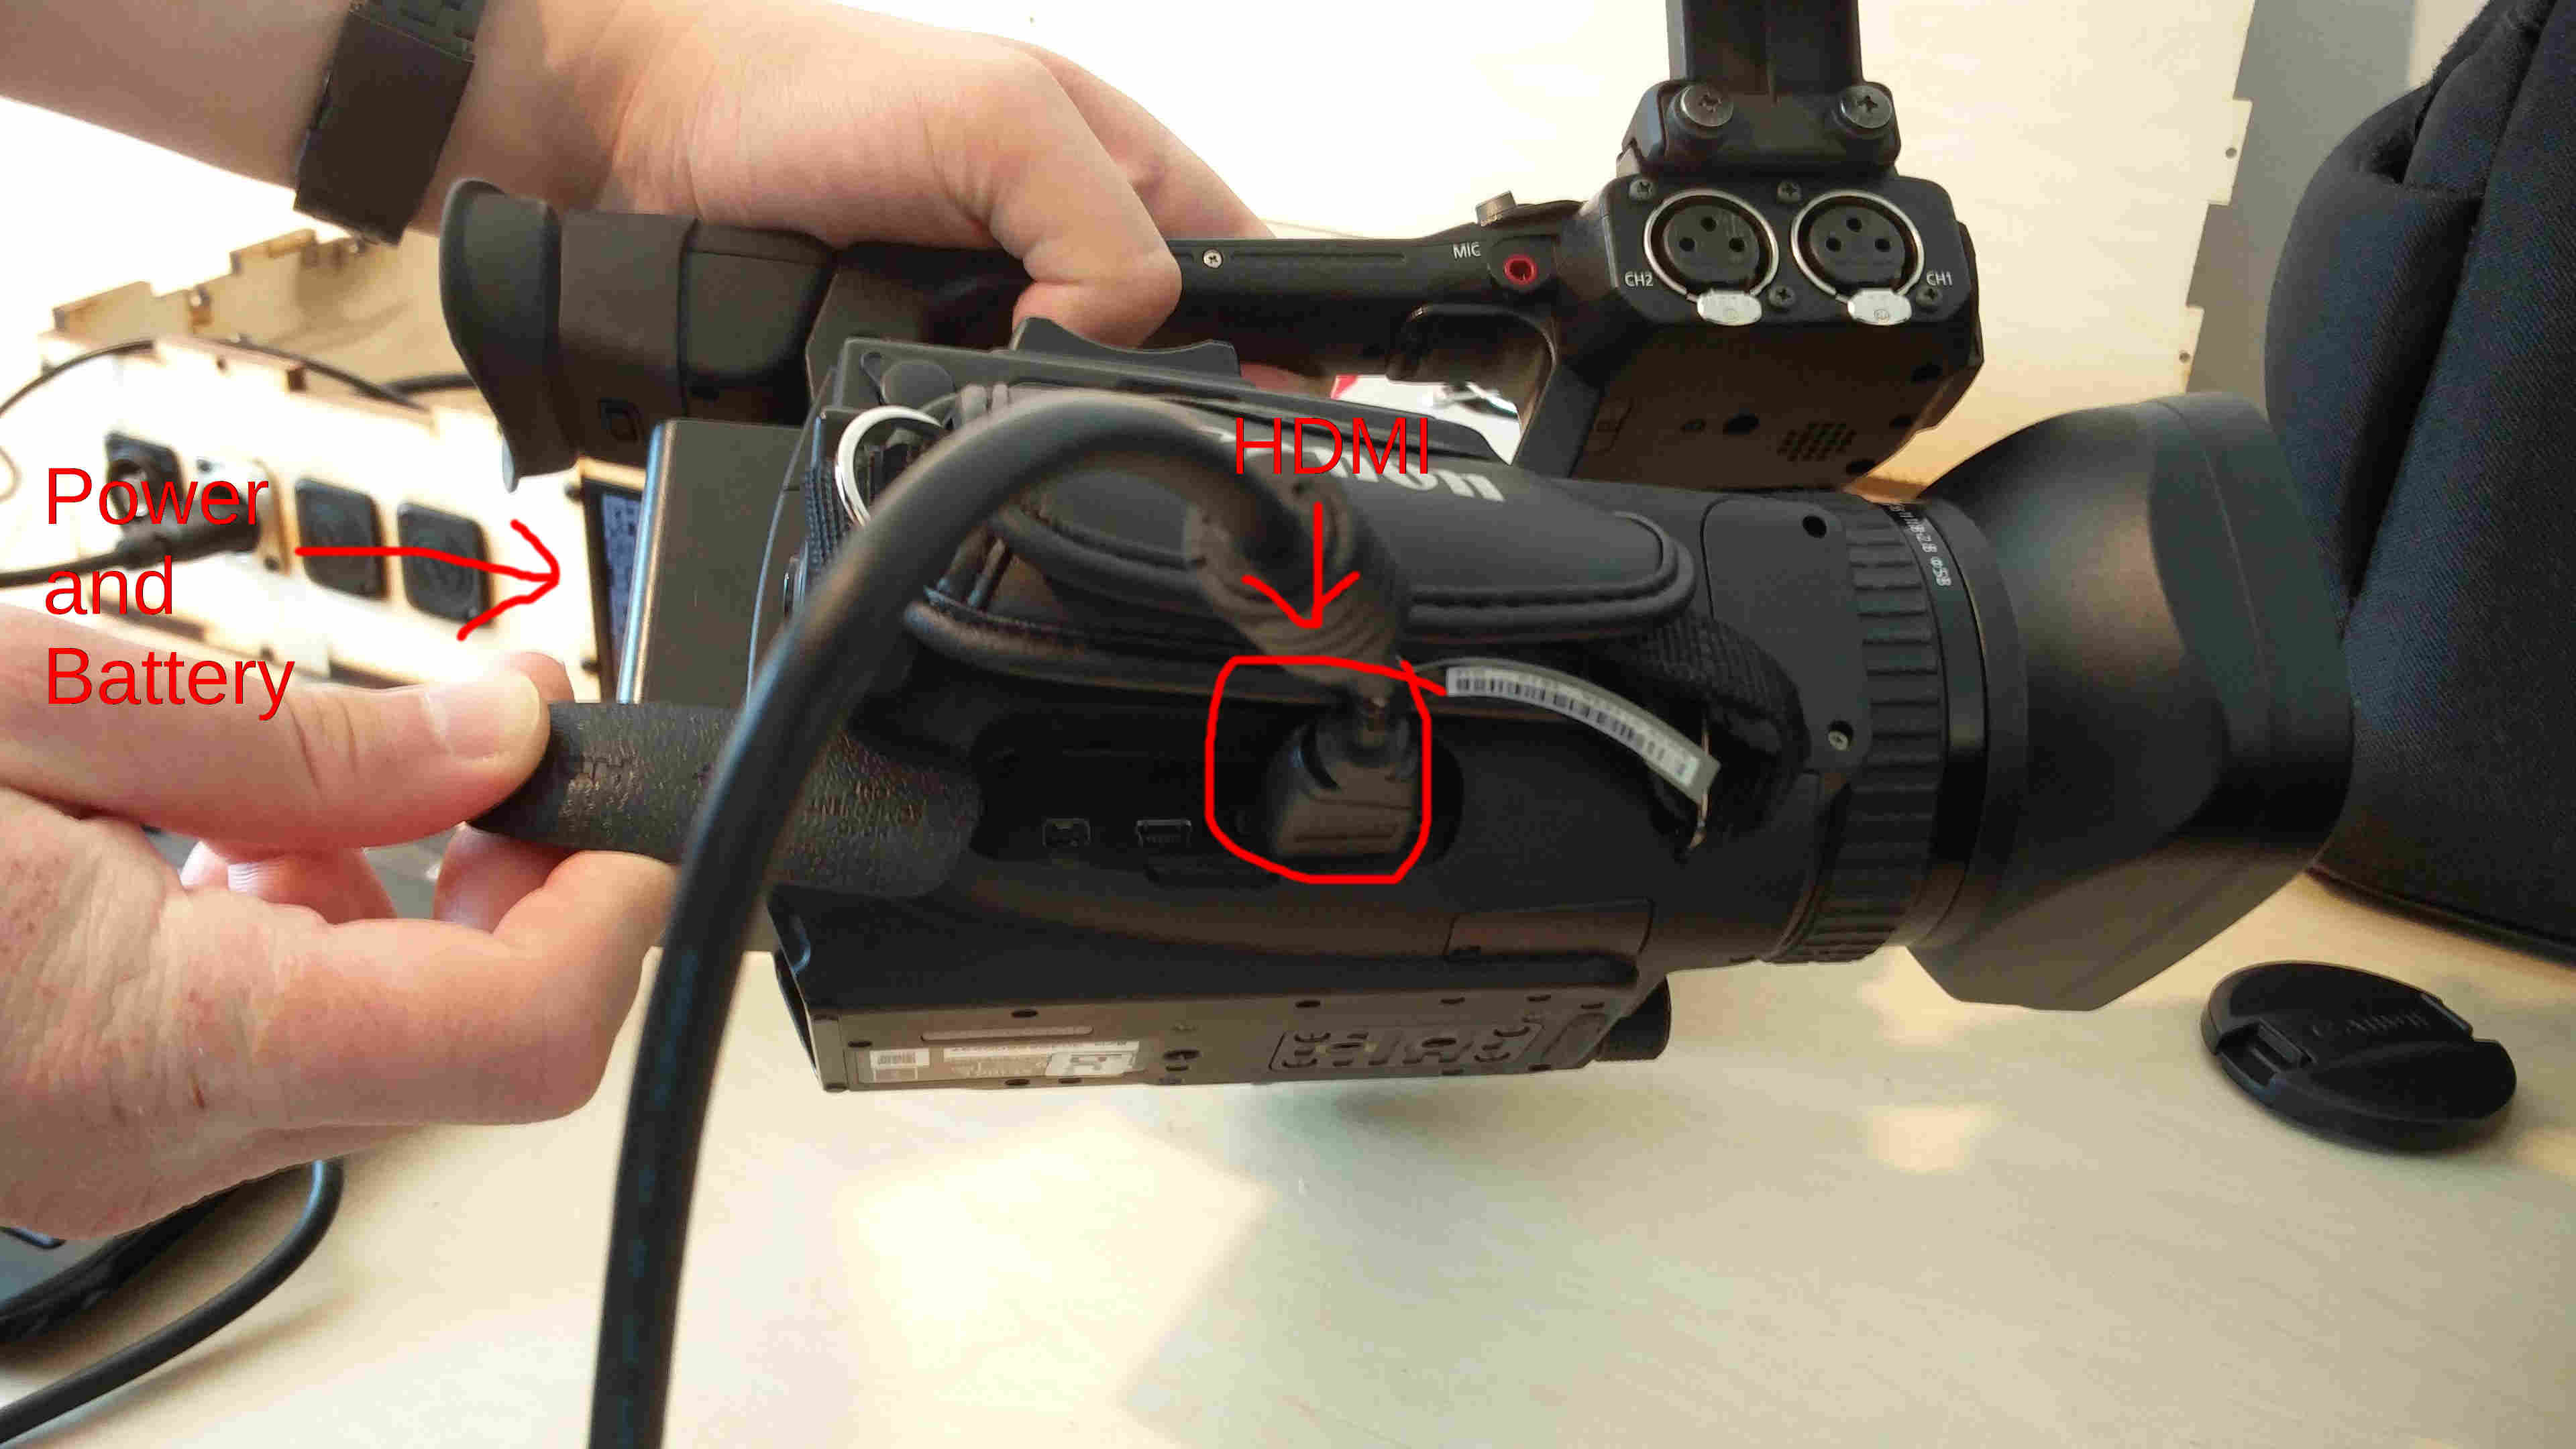
\includegraphics[width = 80mm]{Canon01.jpg}

\subsubsection{Pluggin in the Microphone}
Now plug in the XLR cable of the audio system in CH2.

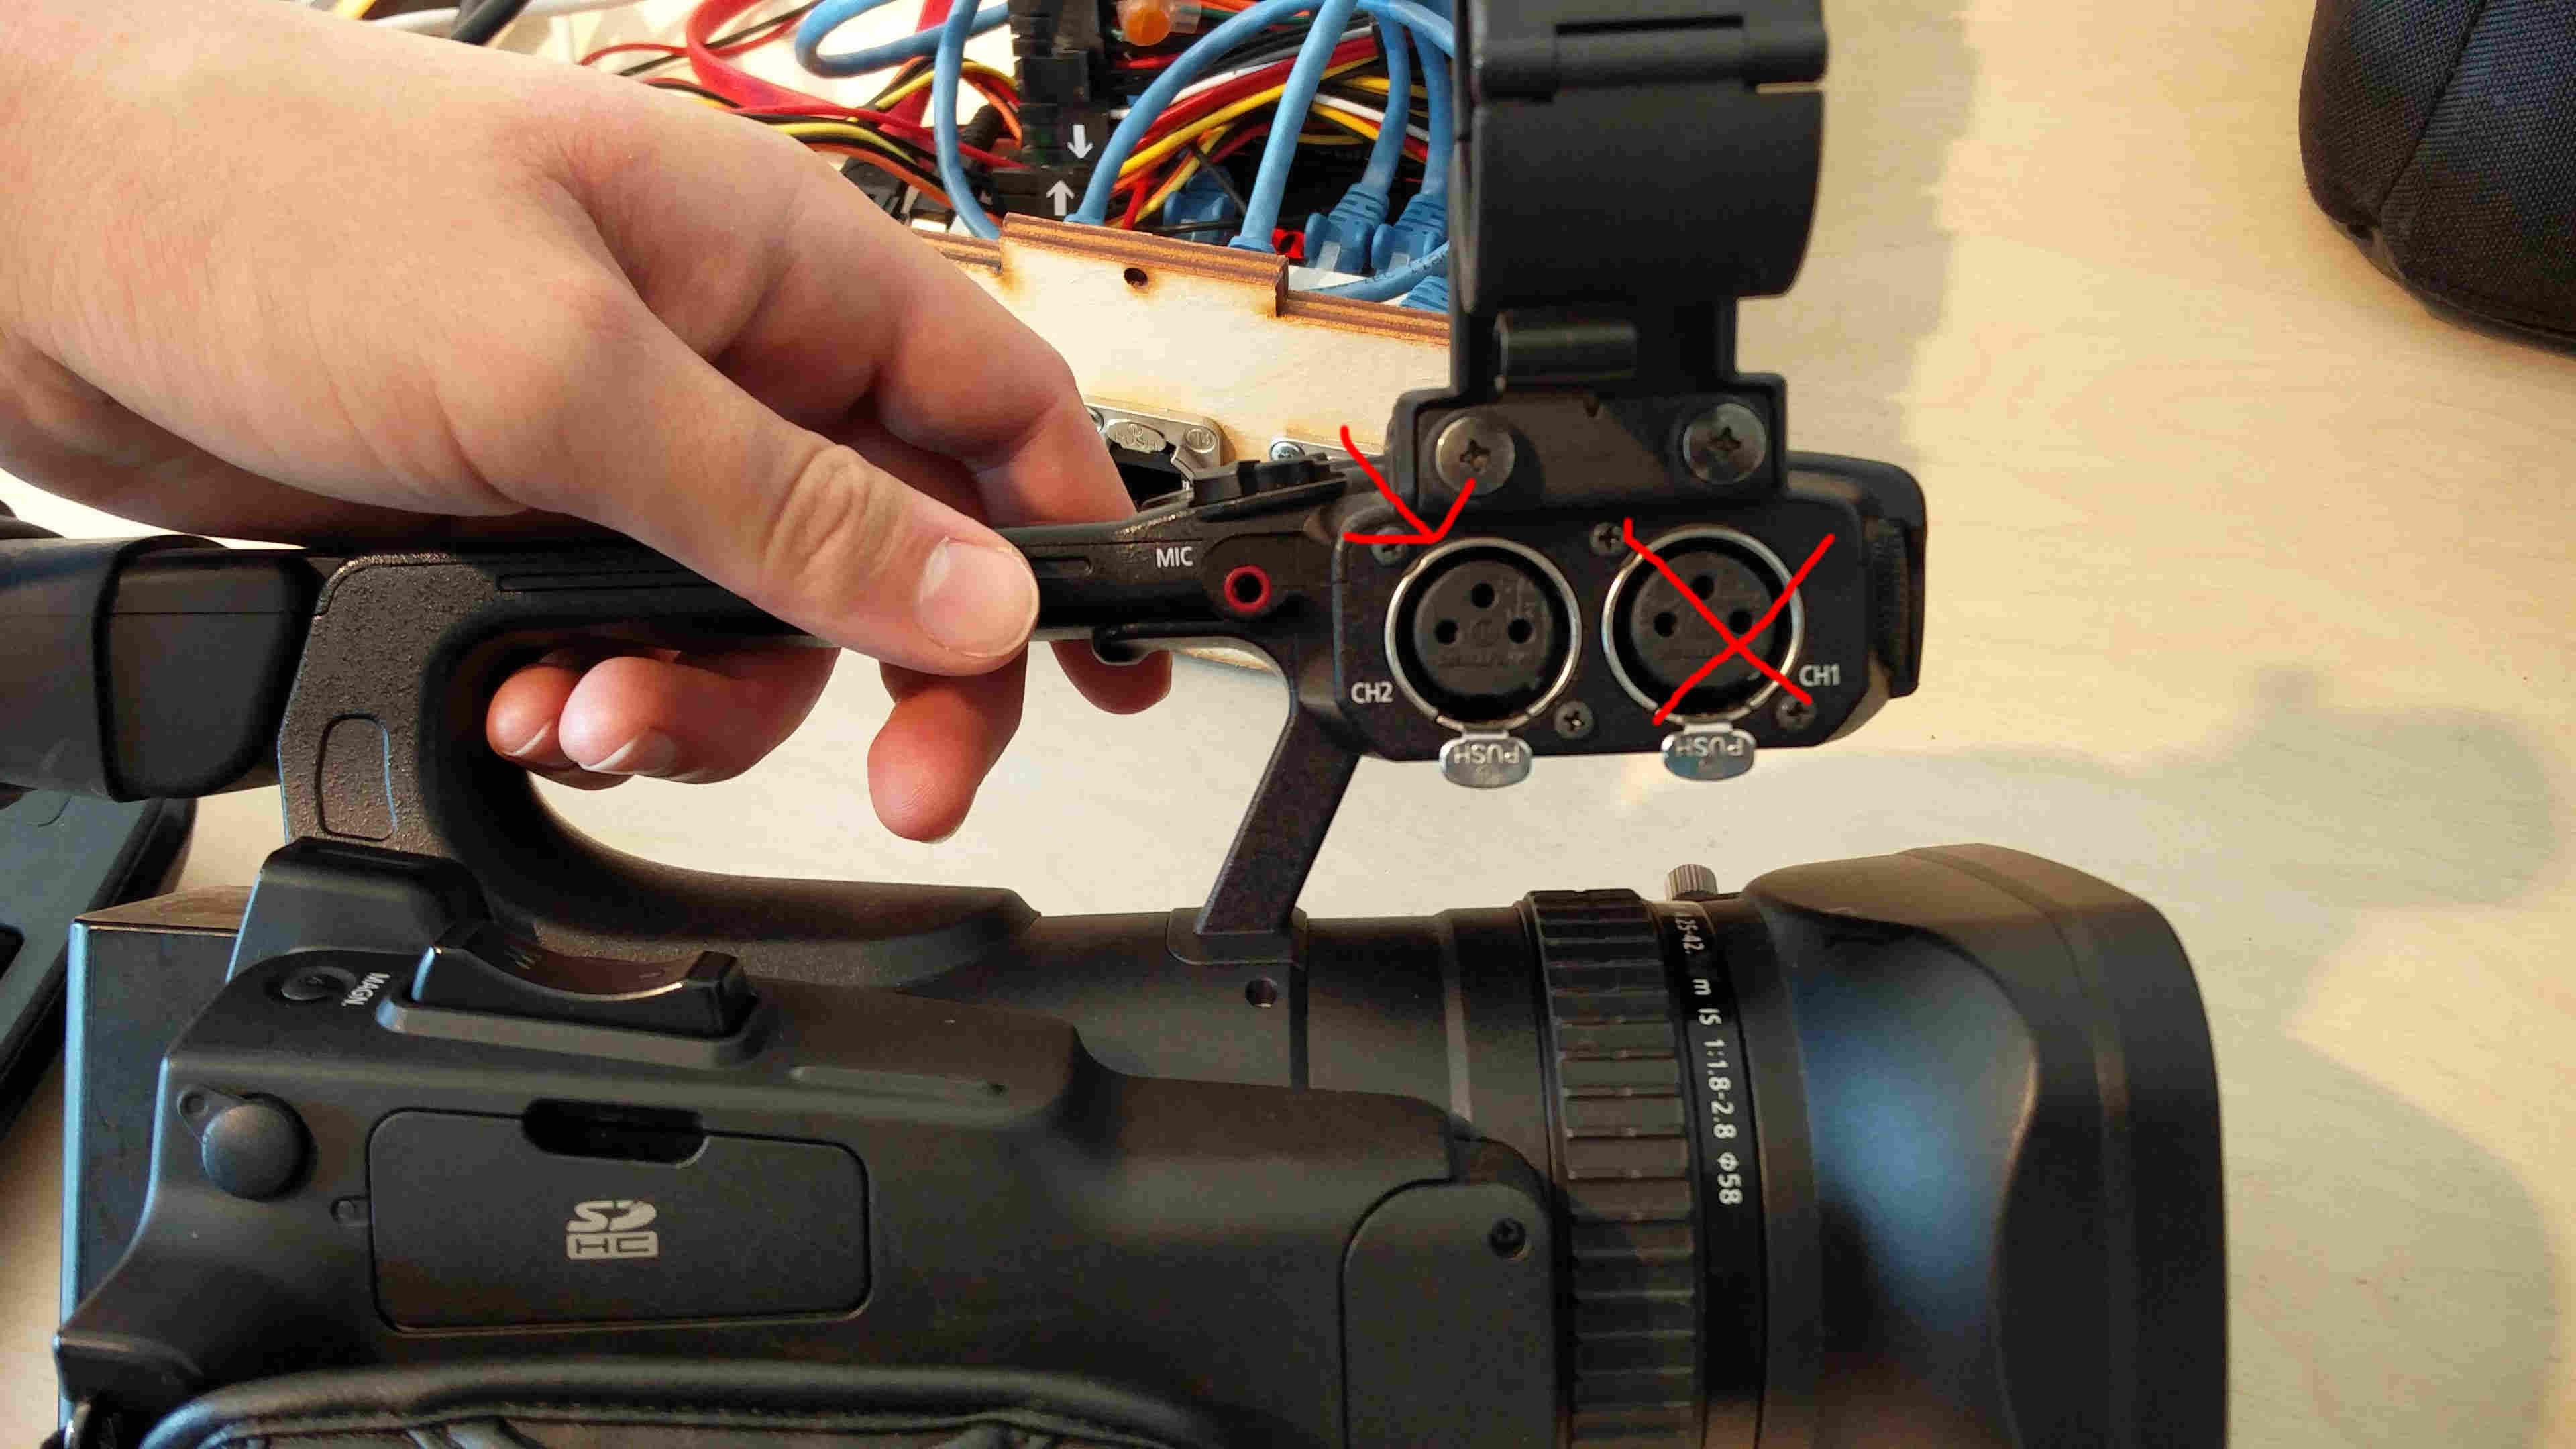
\includegraphics[width = 80mm]{Canon02.jpg}

\subsubsection{Turn on the camera}
You can find the power button at the left side of the camera (looking from behind). The power button should be easy to spot on "top" of the side.

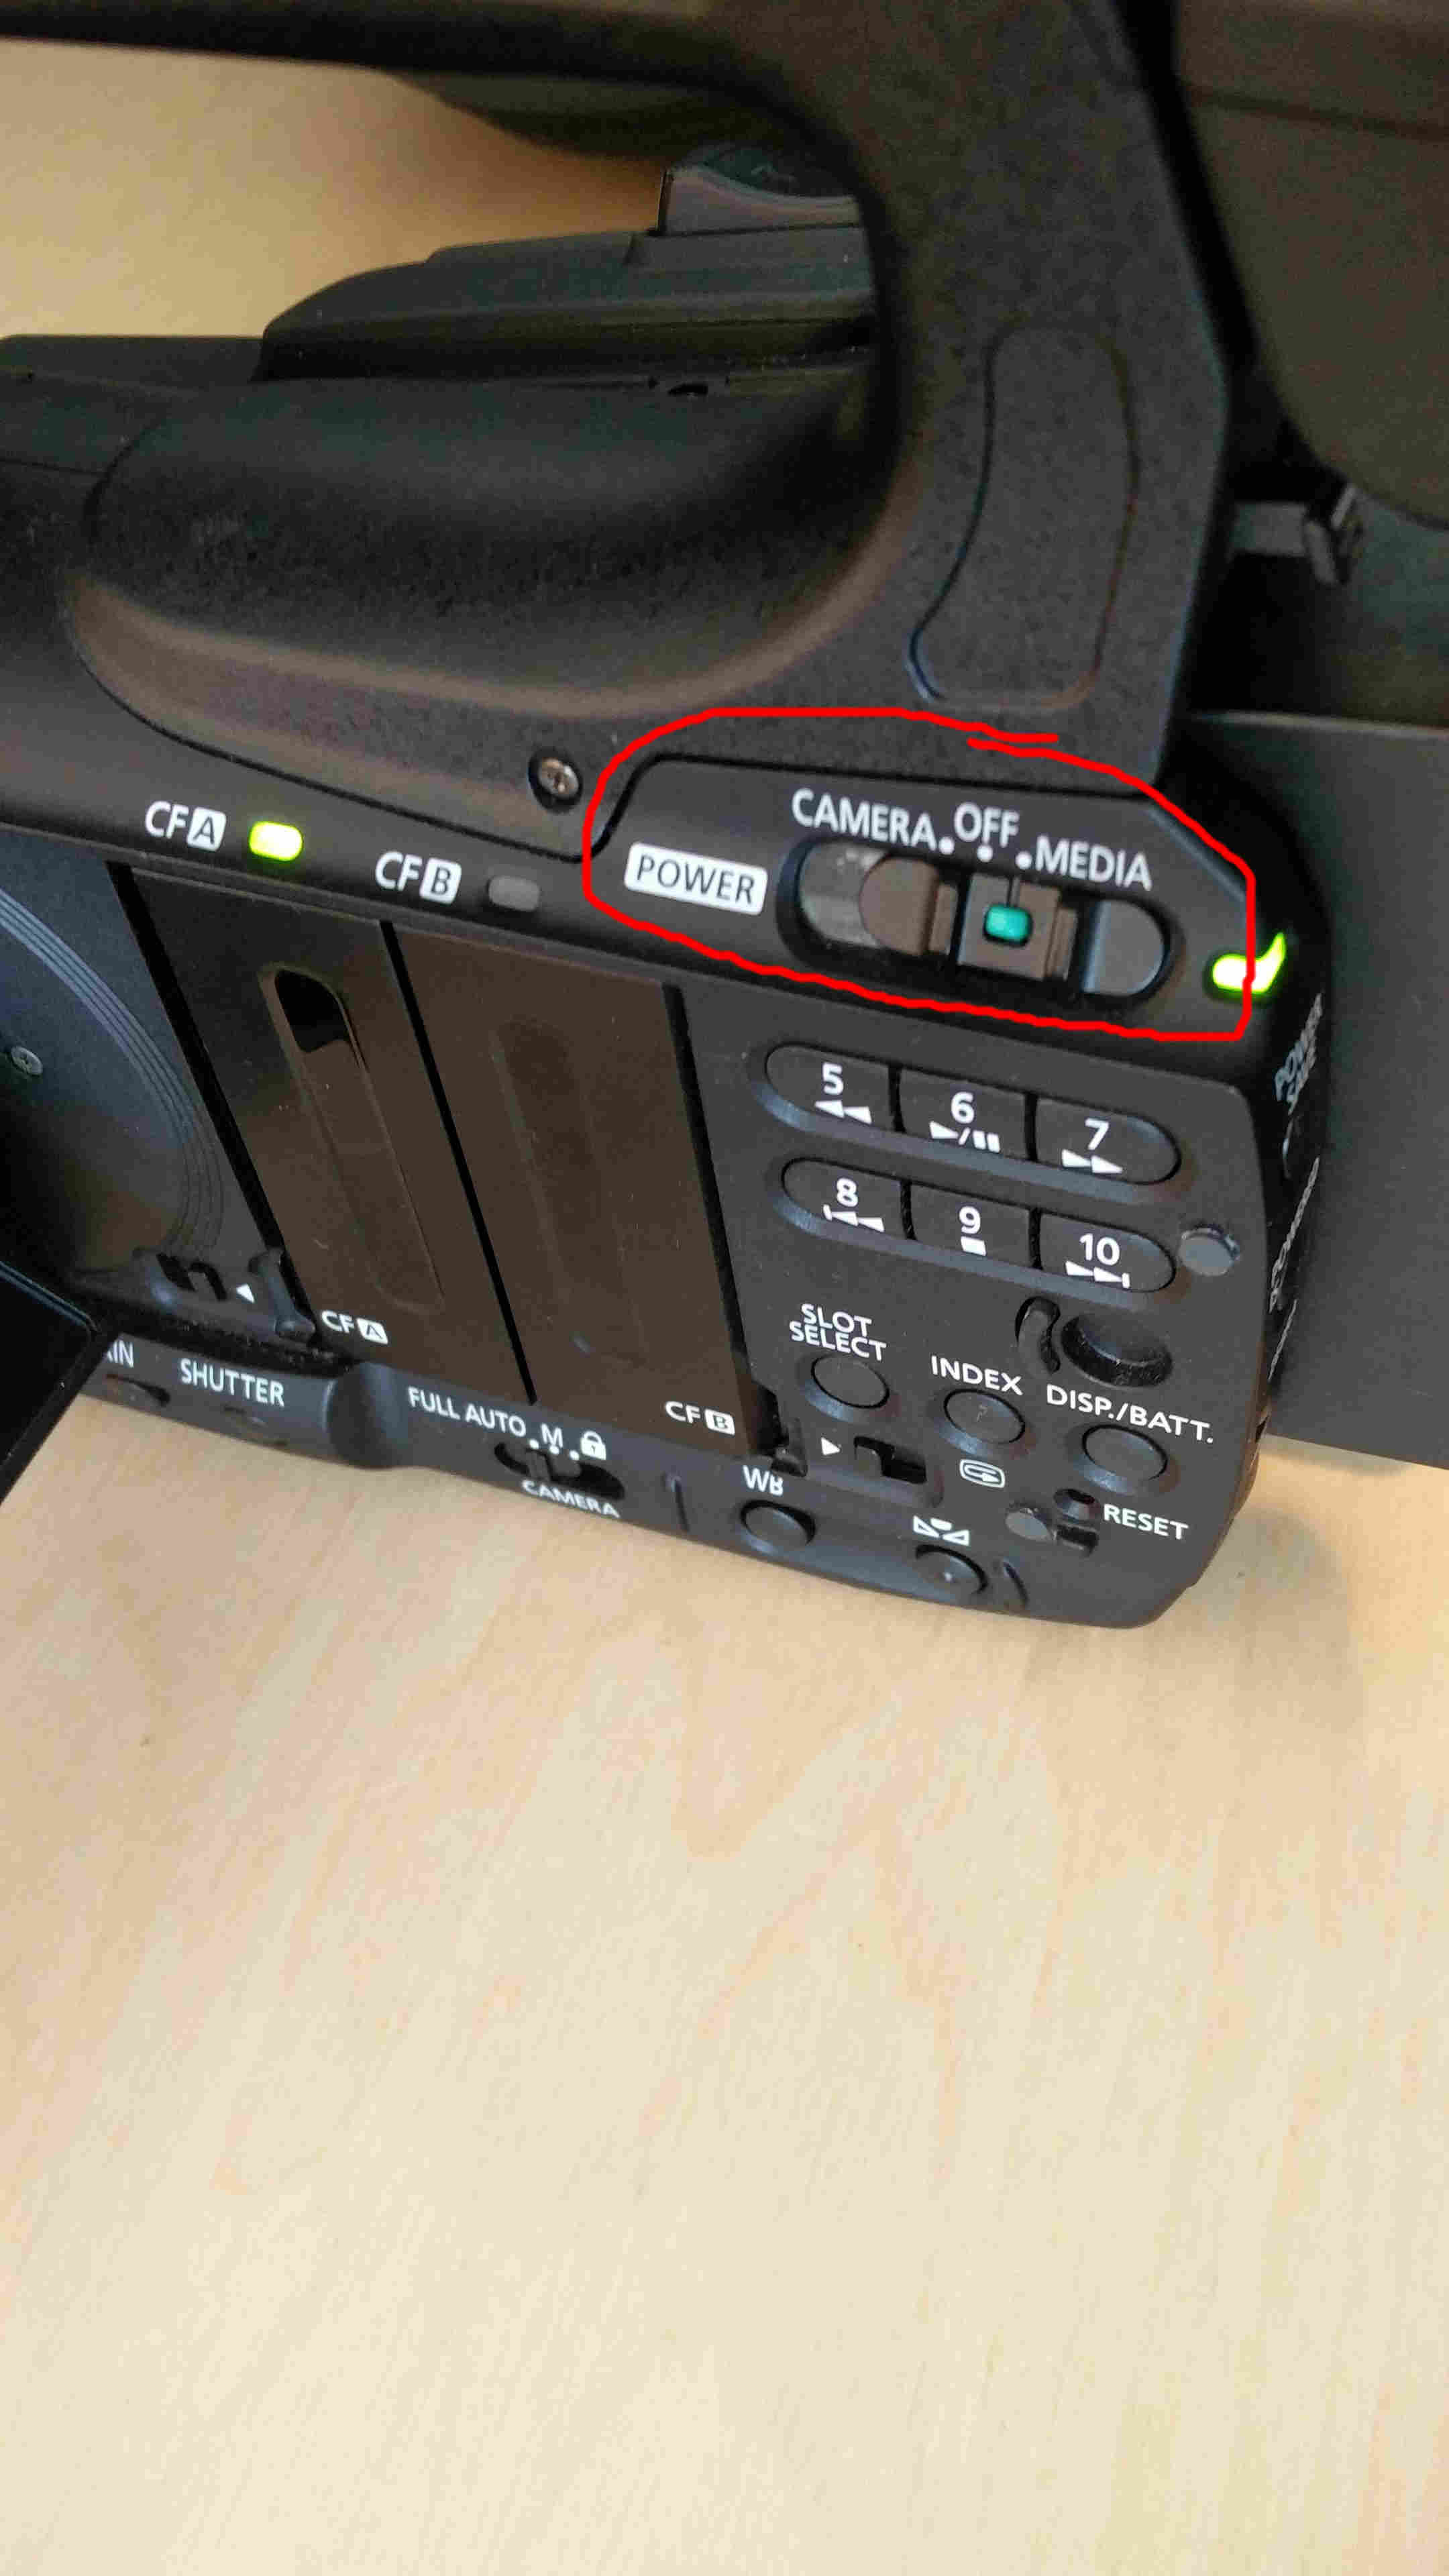
\includegraphics[width = 80mm]{Canon03.jpg}

\subsubsection{Audio settings}
The audio settings can only be done through the actual switches on the camera. Please verify if you've done them correctly with the image. The dial can be on any setting as the automatic setting of switch under it overrides the dial.

\begin{tabular}{| l || l | l | l | l |}
Input & Top switch & Middle switch & Bottom switch & dial at top \\ \hline
CH1 & LEFT (A) & RIGHT (MIC 48V) & LEFT (INT) & anything \\
CH2 & LEFT (A) & LEFT (LINE) & RIGHT (EXT) & anything \\
\end{tabular}

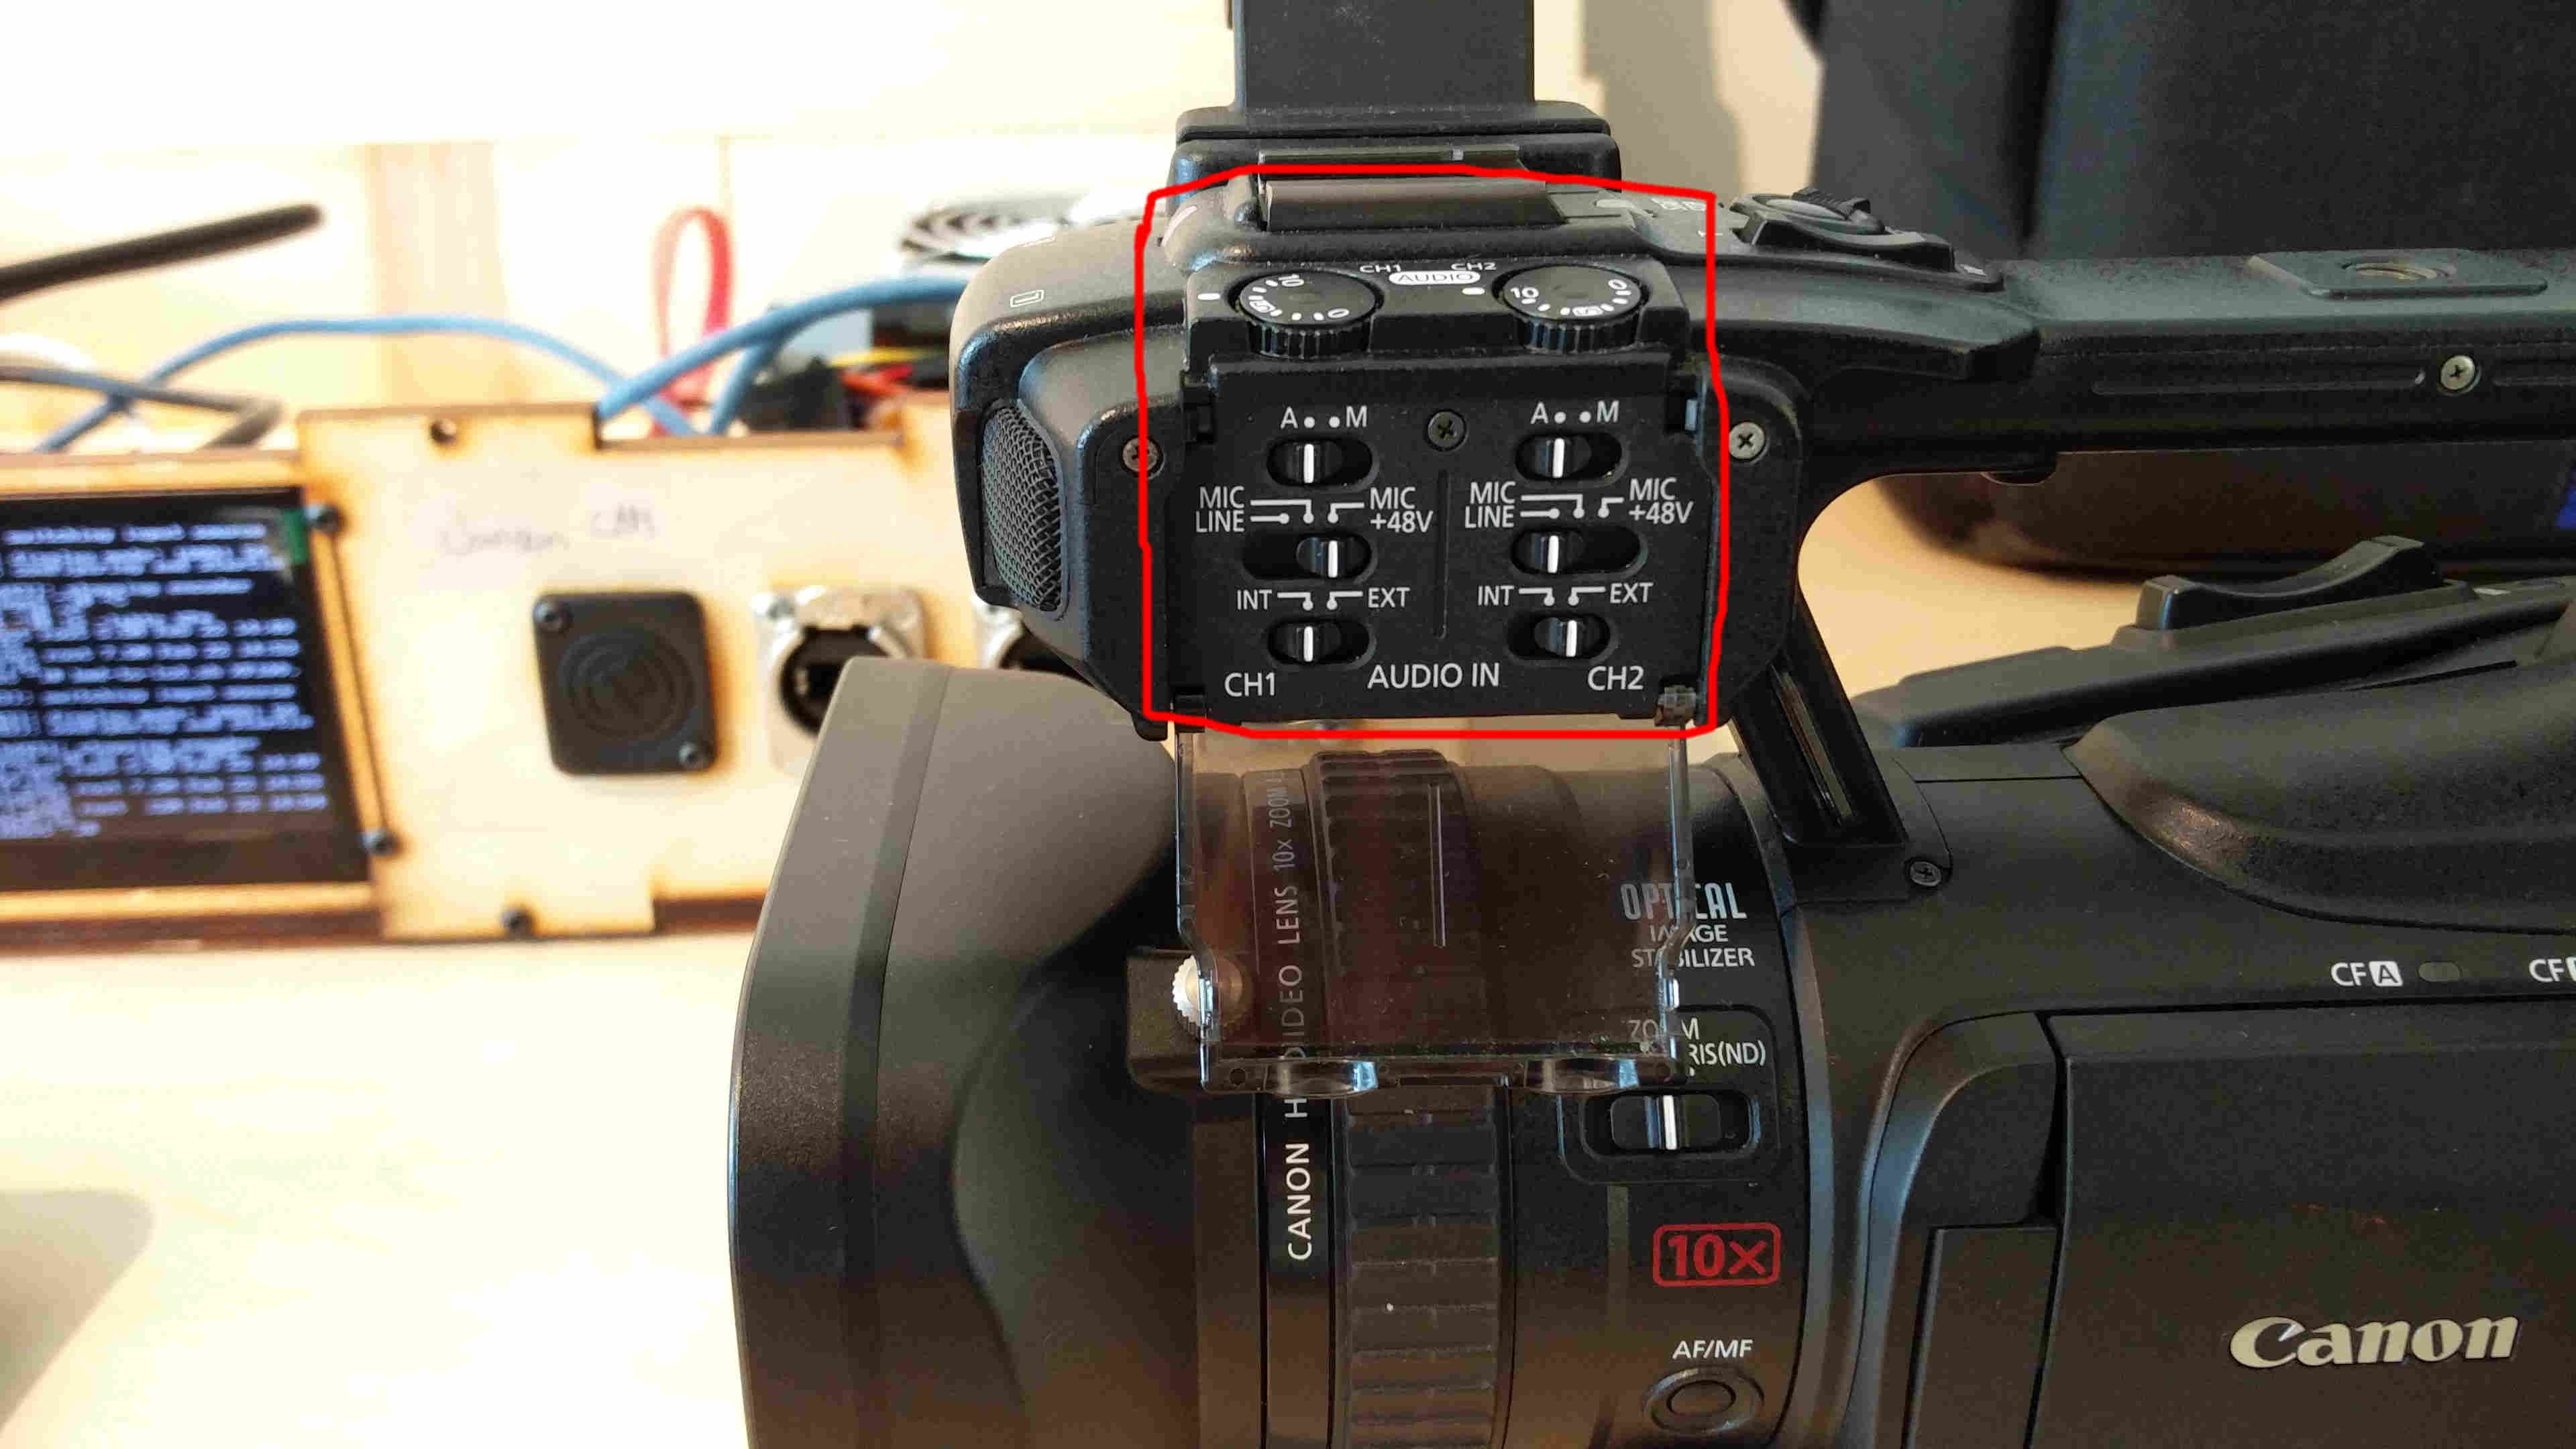
\includegraphics[width = 80mm]{Canon04.jpg}

\subsubsection{Video settings}
The video settings will be done through the onscreen display. The actually focussing and pointing the camera is not your task, it's fine to point it in the general direction afterwards.

You can set the video settings here:

Menu - Last pictogram (wrench) - Bit Rate/Resolution - 1280x720 50Mbps
Menu - Last pictogram (wrench) - Frame Rate - 50P

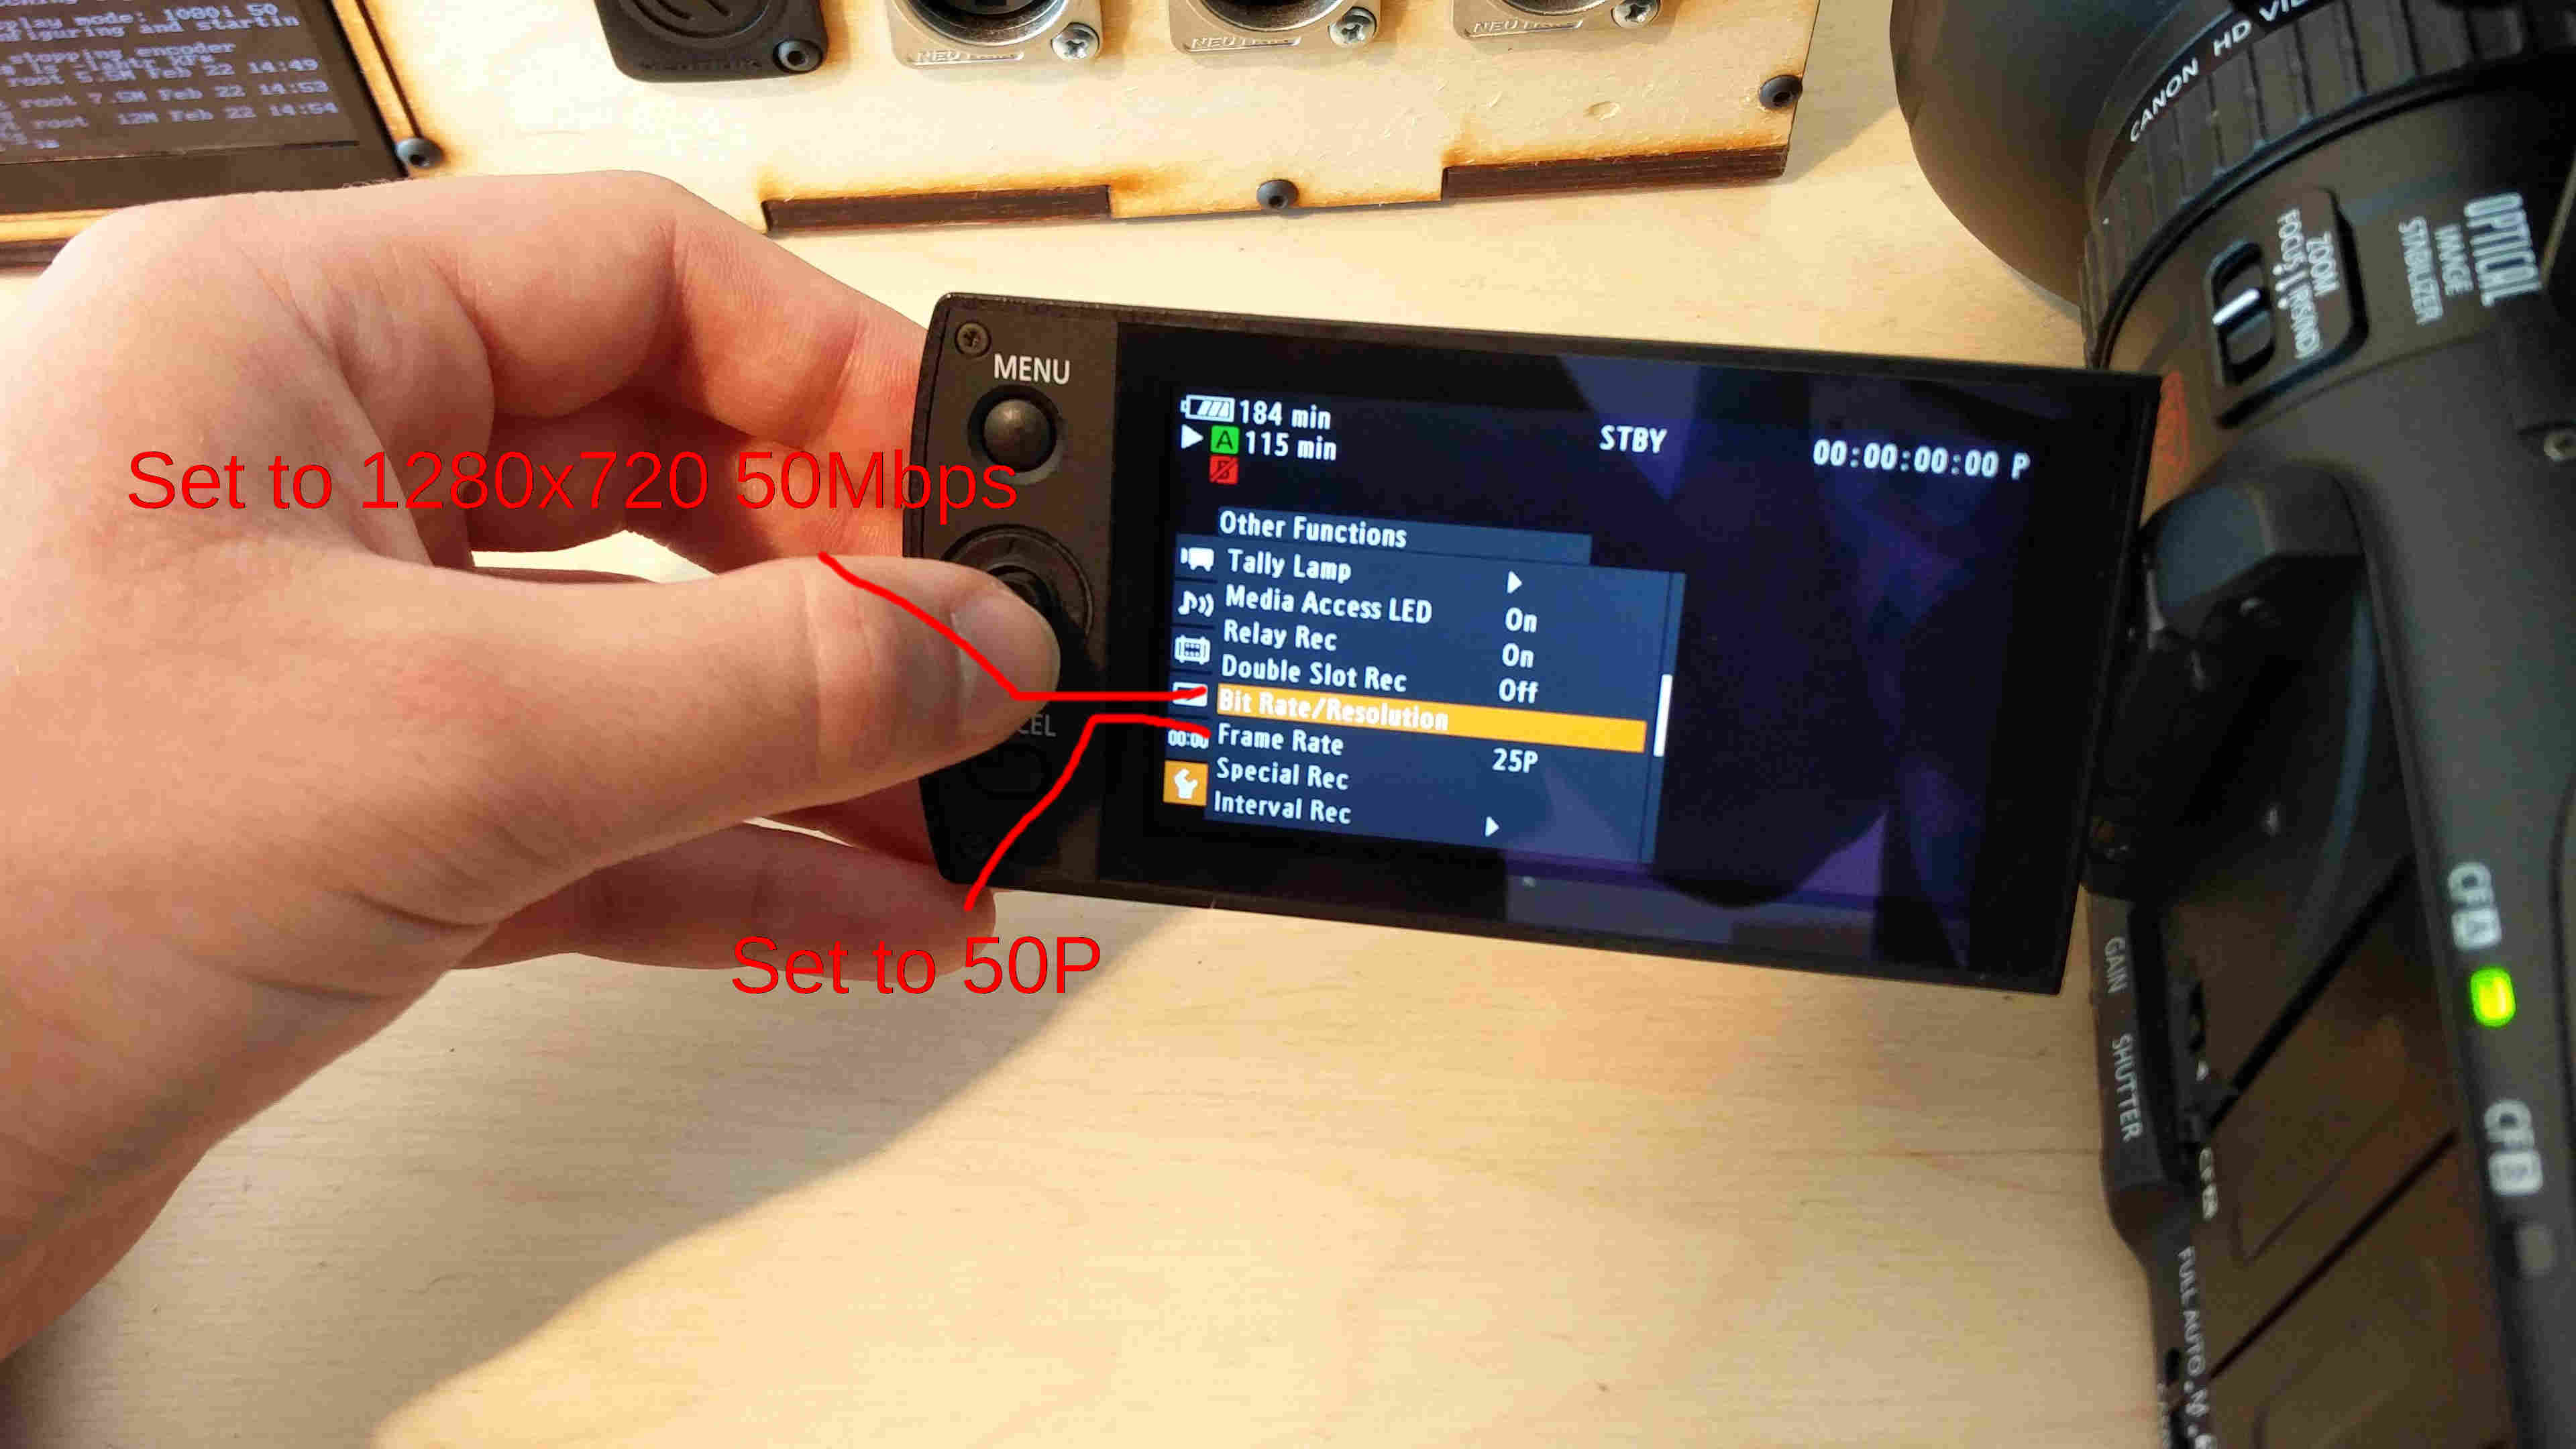
\includegraphics[width = 80mm]{Canon05.jpg}

Unlike the Sony camera, the on screen display actually displays if you've set the correct settings once you're done.
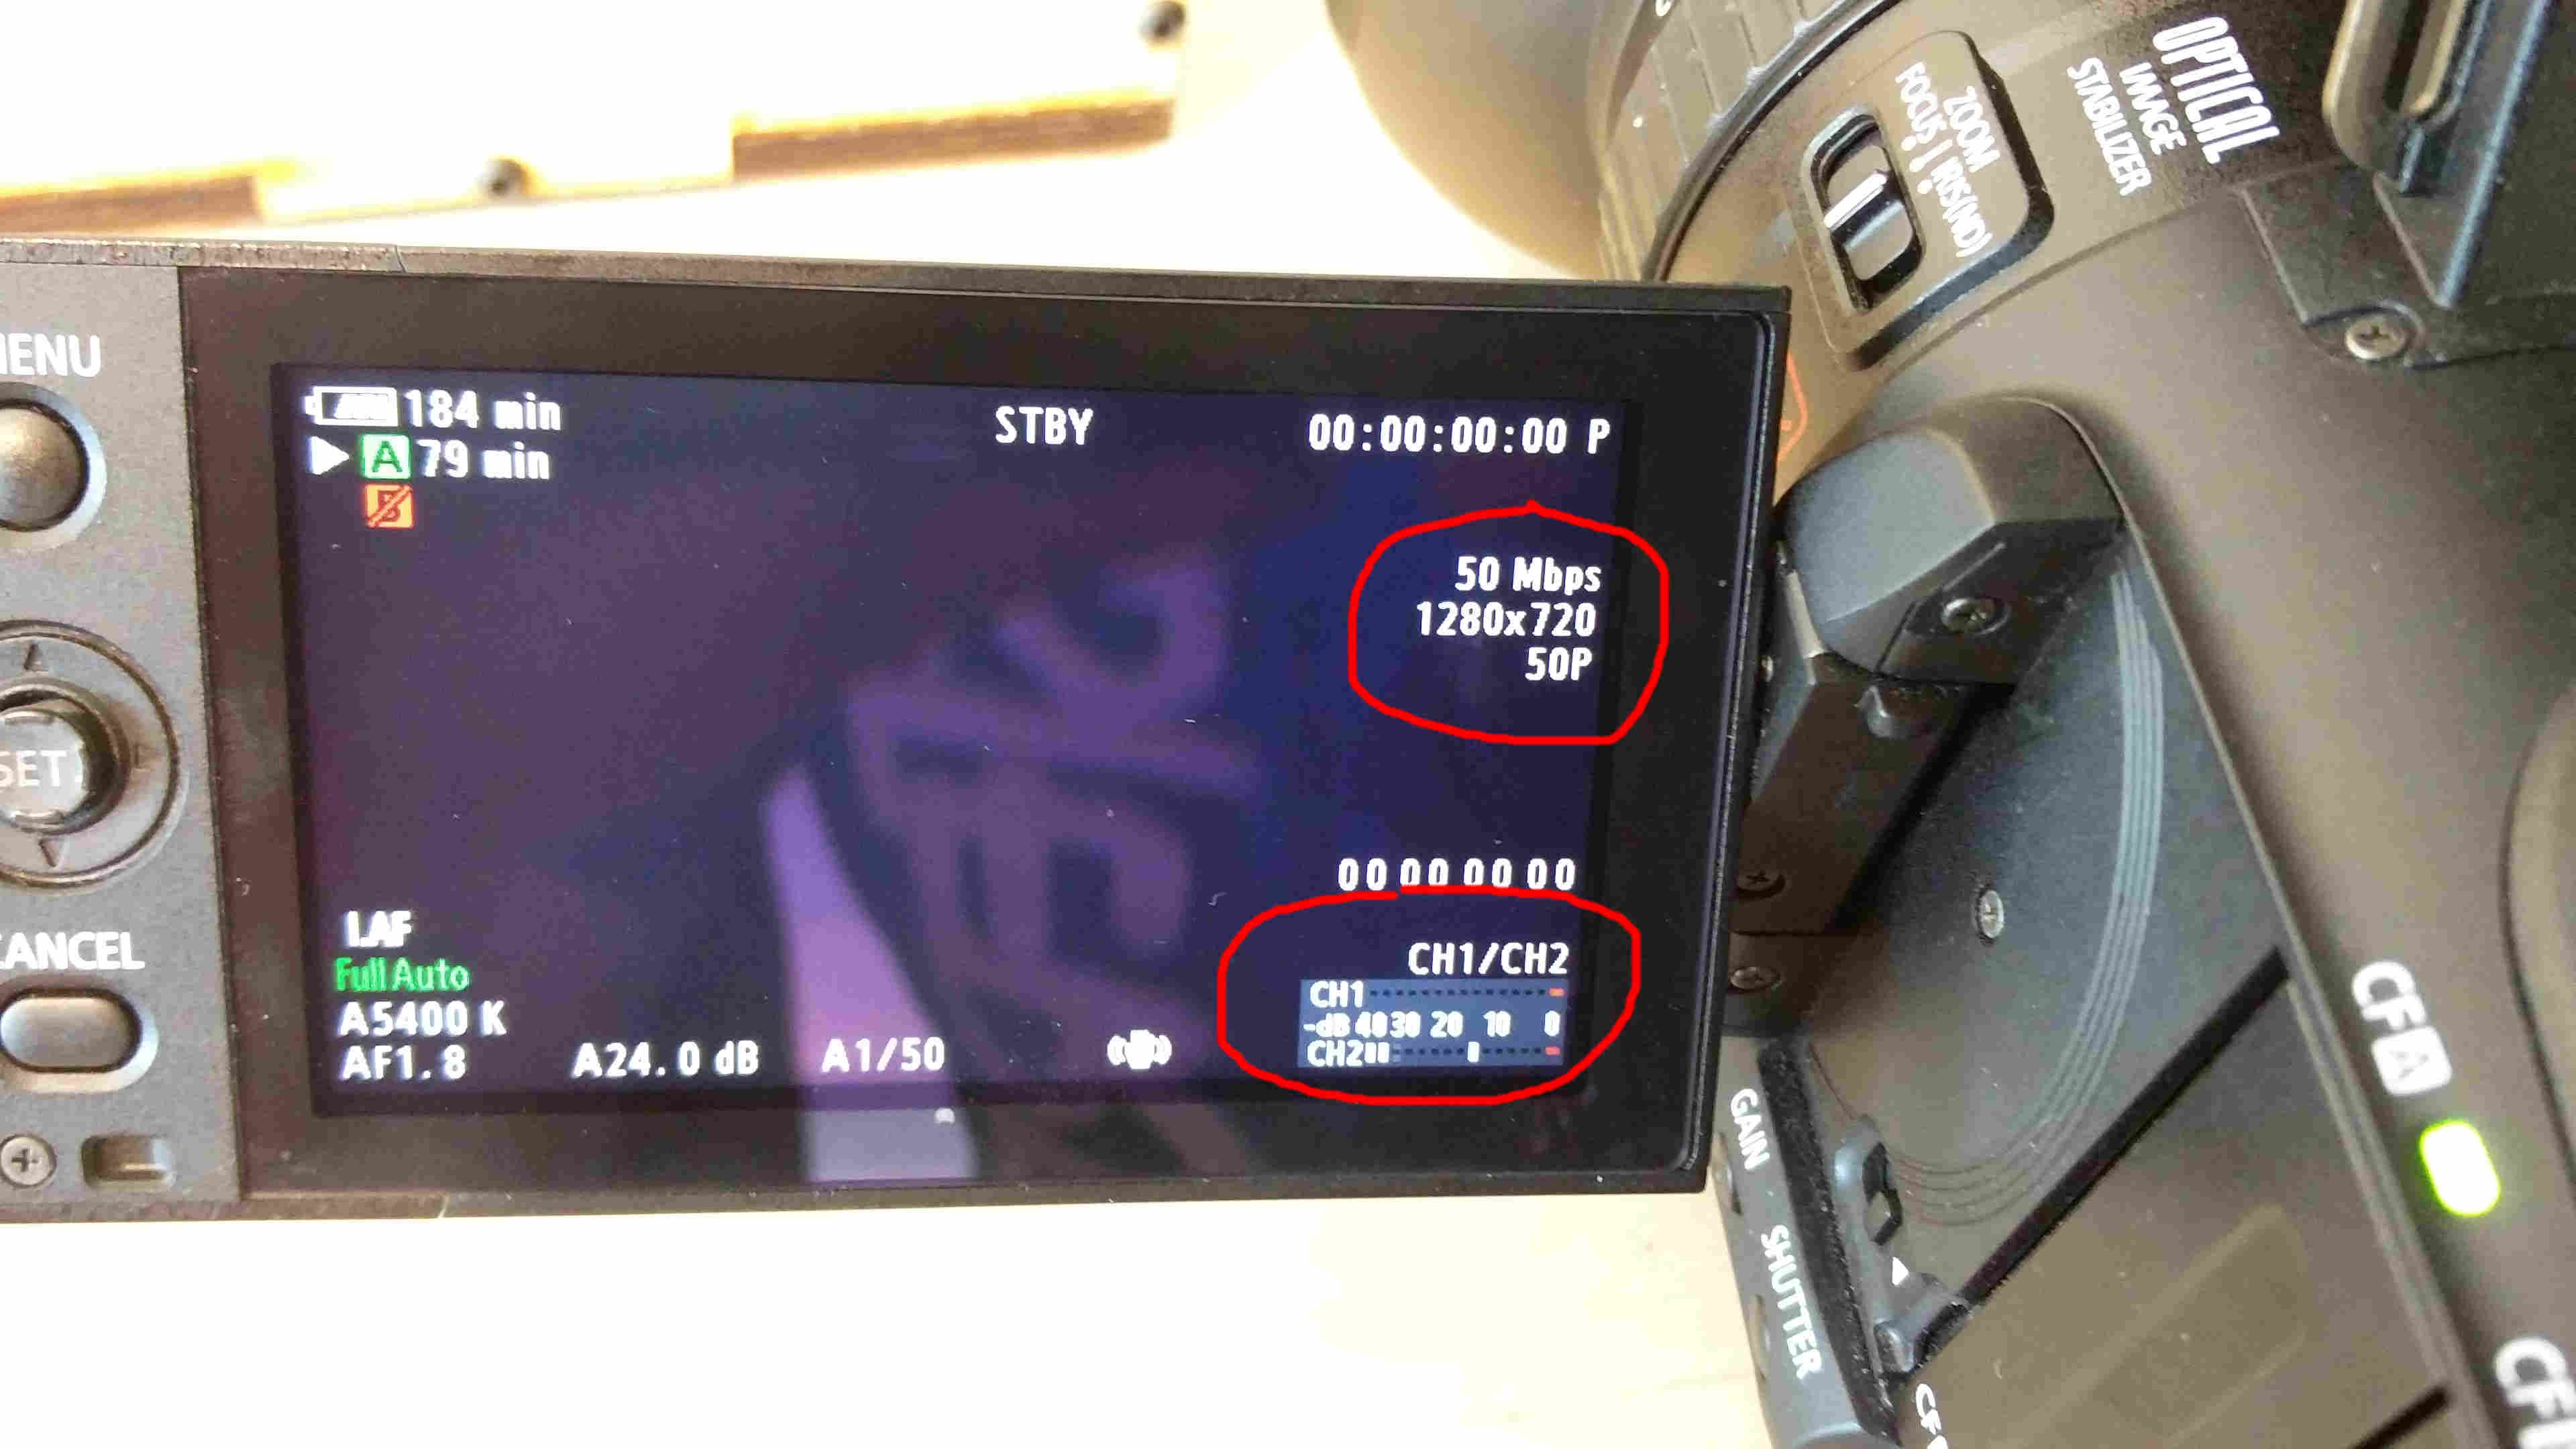
\includegraphics[width = 80mm]{Canon06.jpg}

\subsubsection{Remove the lens cover}
Remove the lens cover.

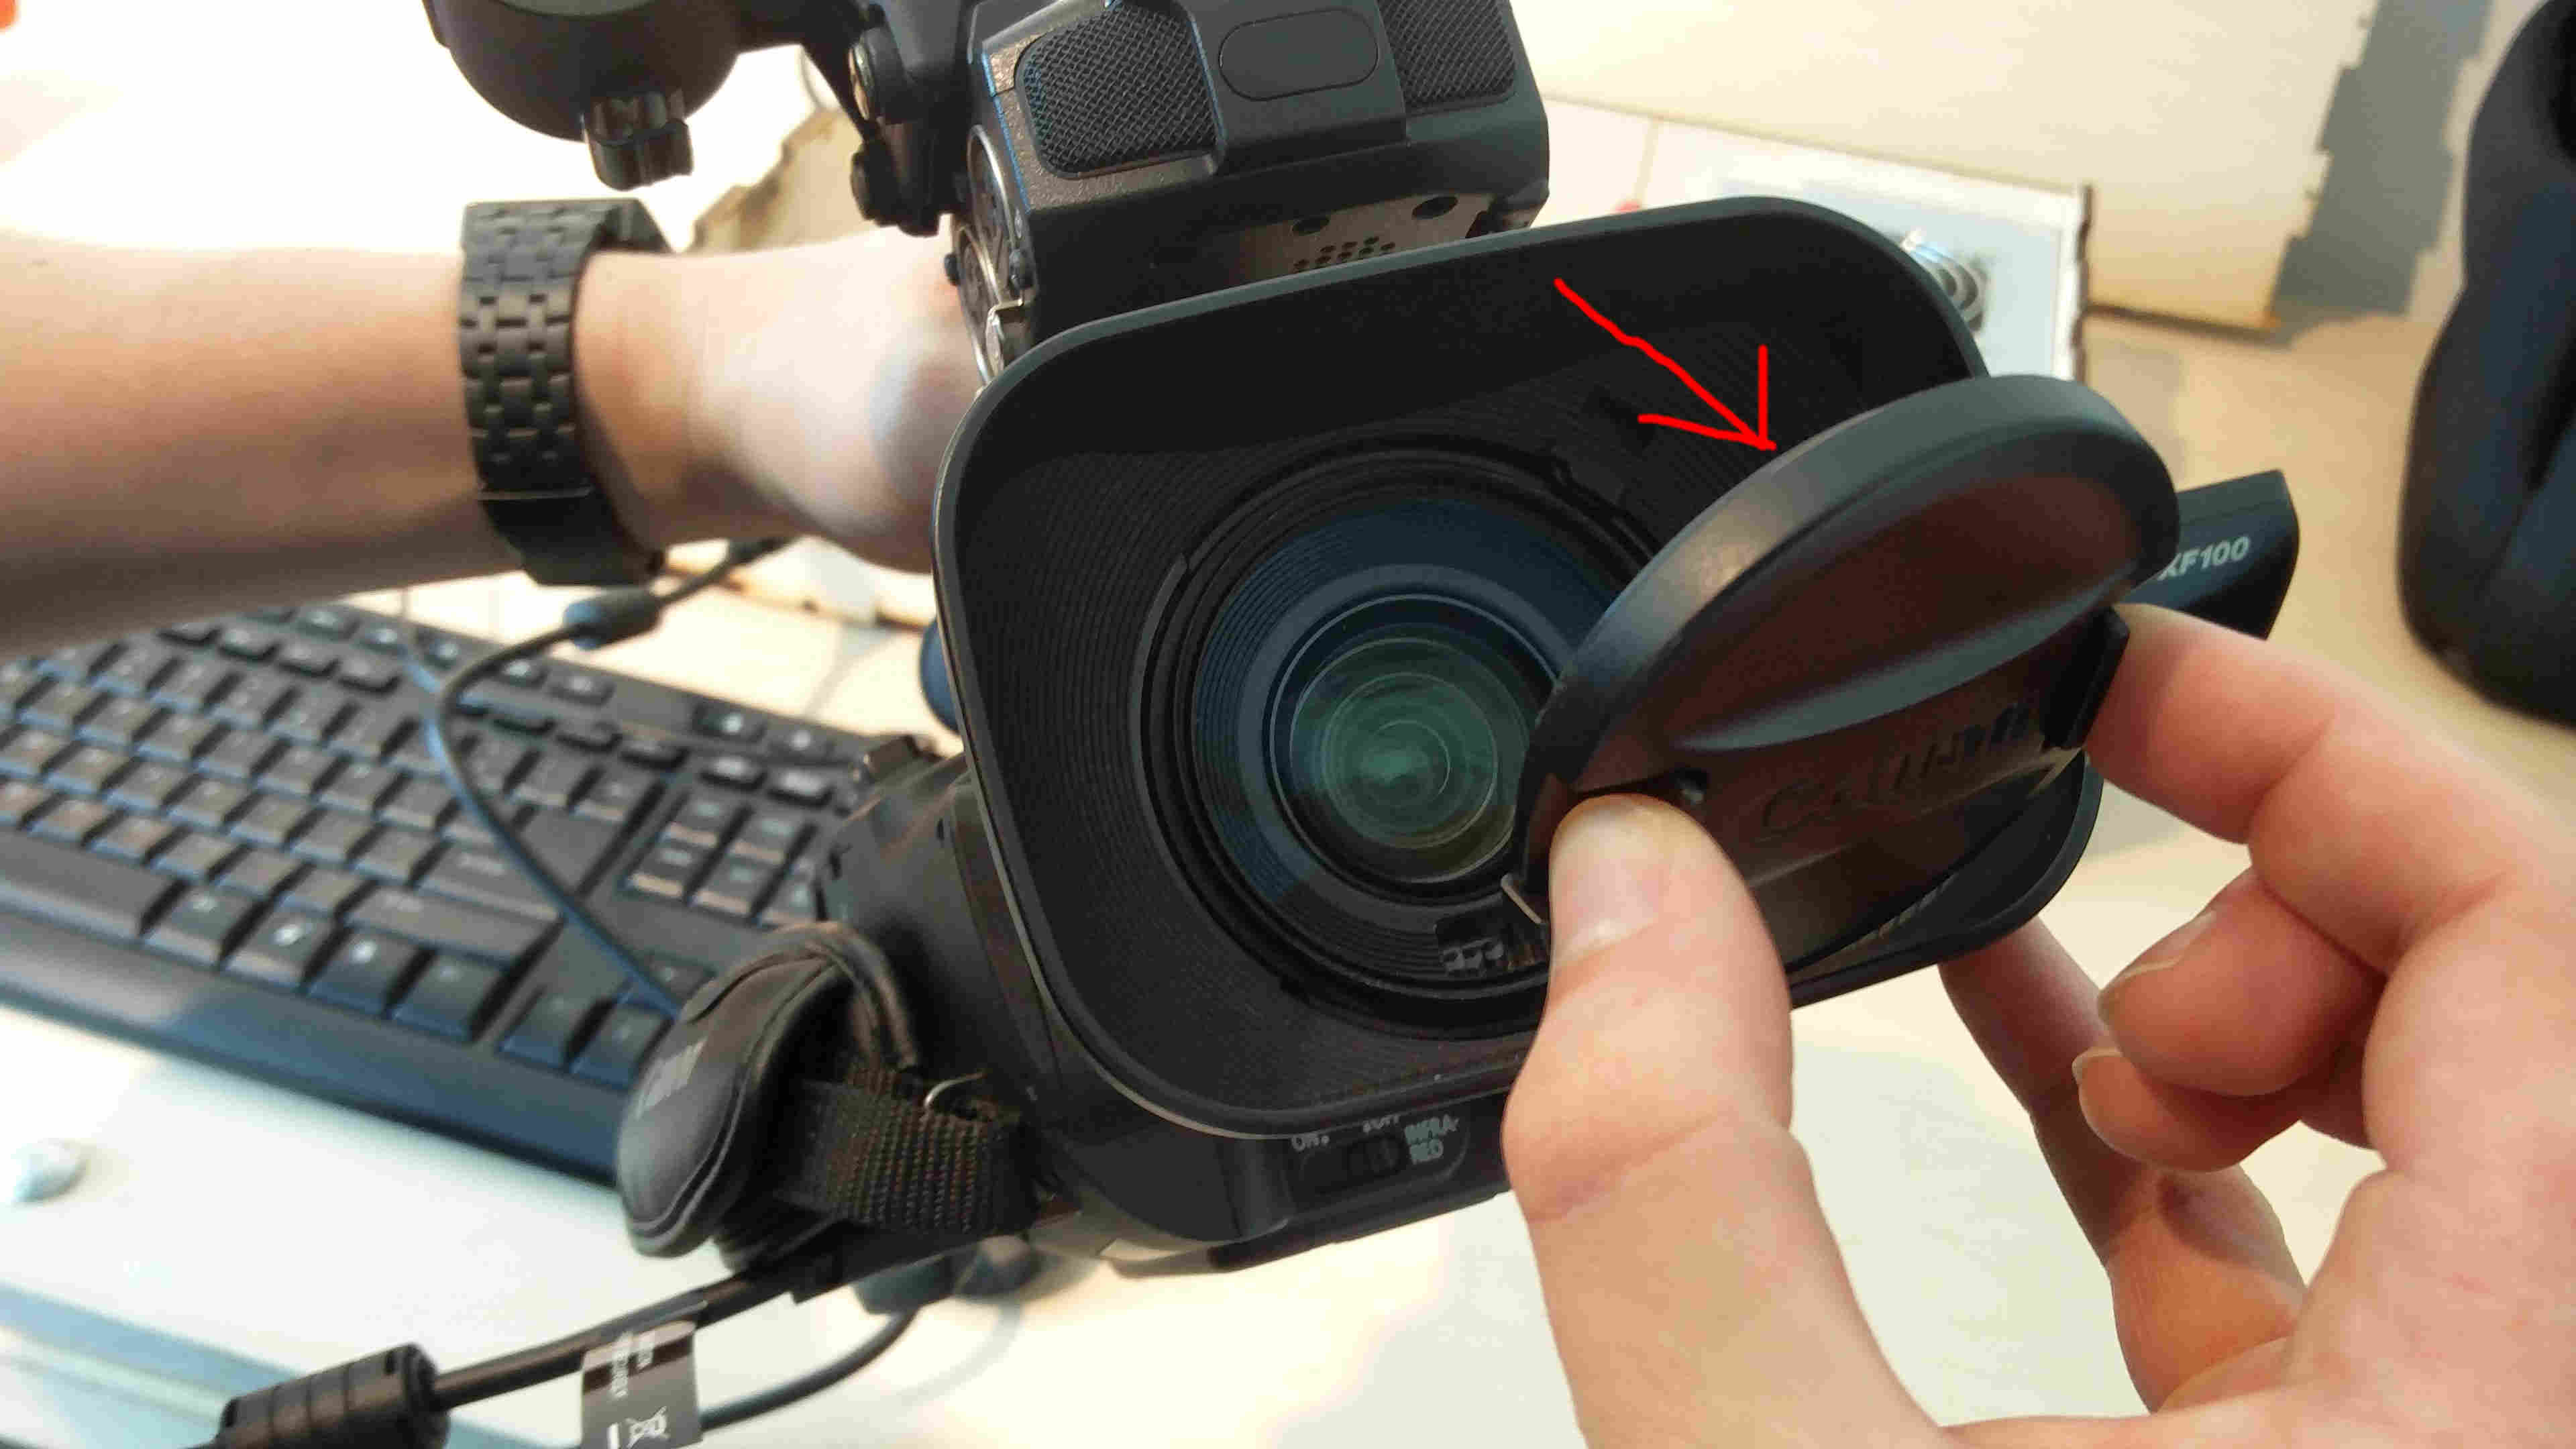
\includegraphics[width = 80mm]{Canon07.jpg}

\subsubsection{Double check}
Please check if the settings have been implemented correctly. 

For audio: you'll see CH1 spike when tapping the camera and CH2 when tapping the speaker microphone, do note that the speaker microphone will have to be turned on for this to work. Alternatively you can grab a headset and CH1 should come out of the left ear and CH2 should come out of the right ear.

For video: You can check the display settings.

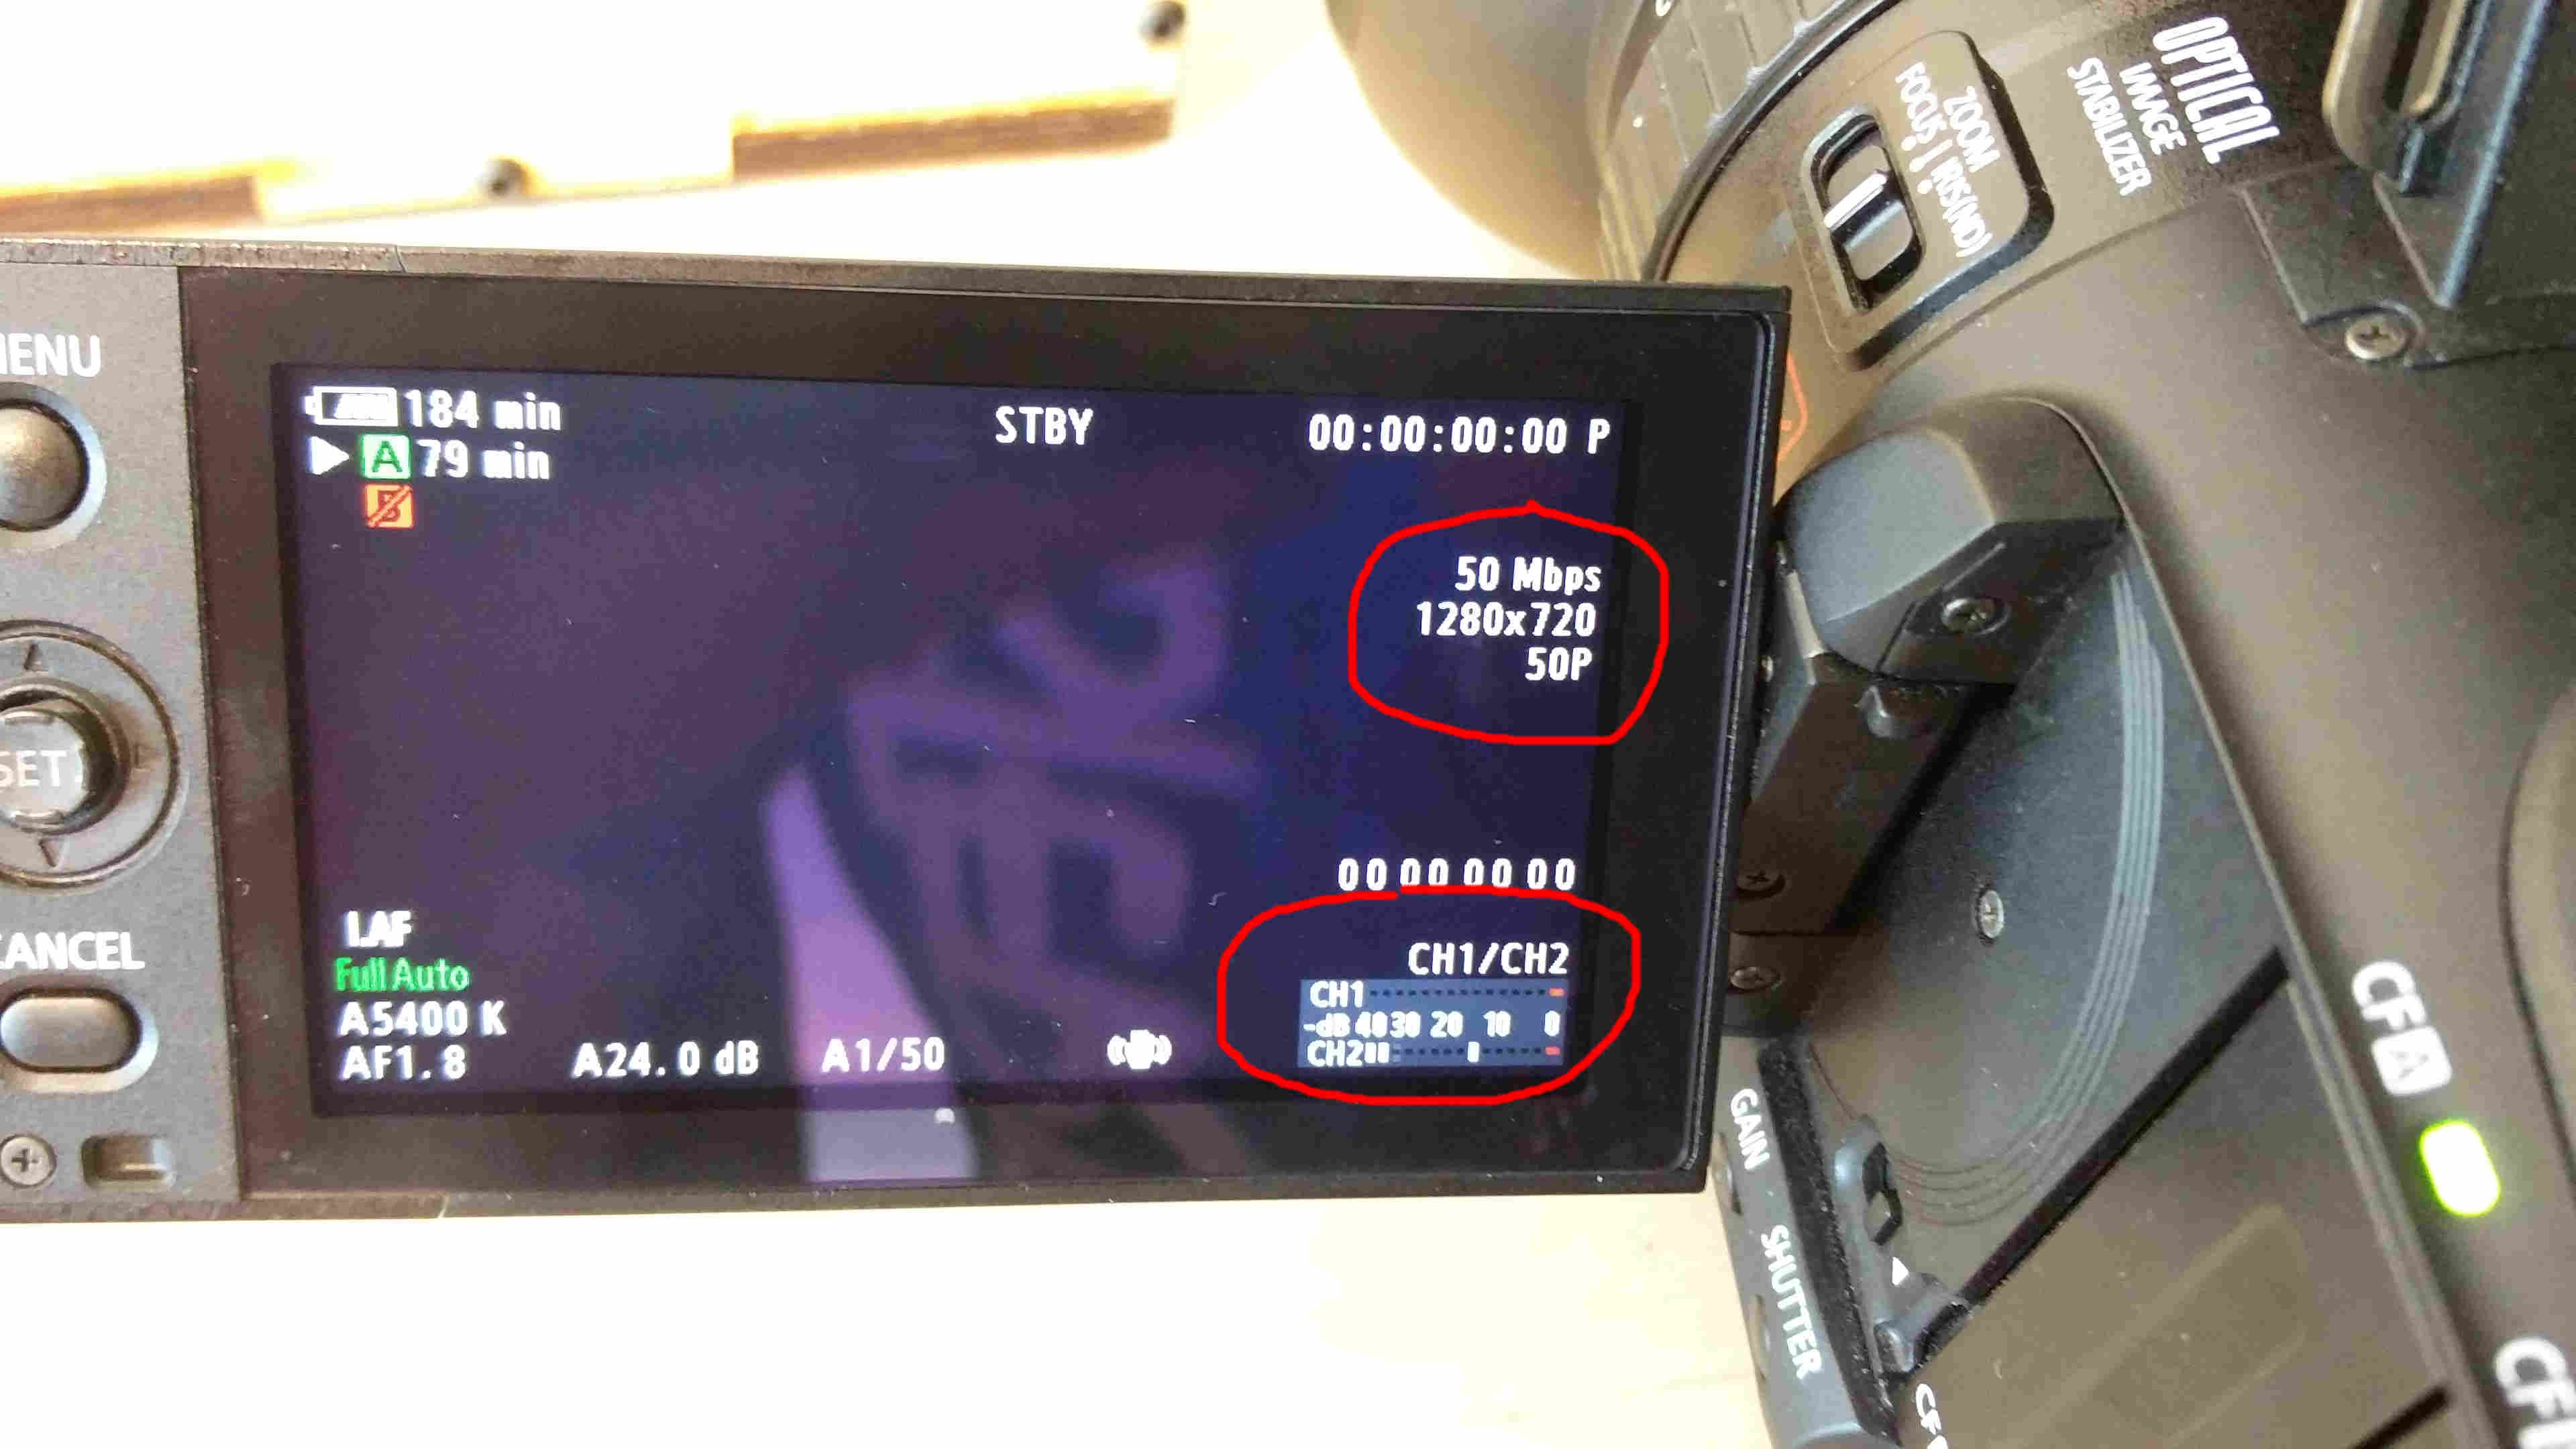
\includegraphics[width = 80mm]{Canon06.jpg}

\subsubsection{Contact control}
Please report that you've finished the room at the assigned control points. They will have the follow-up steps and know what still has to be done in the building.


\end{document}
 
